\documentclass[conference]{IEEEtran}

\usepackage{graphicx}
\usepackage{multirow}
\usepackage{amsmath, amssymb}
\usepackage{hyperref}
\usepackage{subcaption}
\usepackage{caption}
\usepackage{cite}
\usepackage{float}
\usepackage{algorithm}
\usepackage{algorithmic}

\title{D.I.A.G.R.A.M.: Digital Image Analysis for Graph Recognition And Modeling}

\author{
    \IEEEauthorblockN{Filippo Garagnani, Saverio Napolitano, Nicola Ricciardi}
    \IEEEauthorblockA{
        'Computer Vision and Cognitive System' course \\
        \textit{Università di Modena e Reggio Emilia}
    }
}

\begin{document}

\maketitle

\begin{abstract}
This report describes D.I.A.G.R.A.M., a system for diagram recognition and generation. We present its architecture, the logic behind deterministic algorithms and the training of its deep learning components. The project aims to transform visual diagram input into structured representations.
\end{abstract}

\section{Introduction}
Diagrams are crucial in education, documentation, and many other fields. Developing a system that automatically understands and generates diagrams may reveal helpful for having high-quality, easily editable representations. This, however, poses challenges involving classification, shape detection, structure interpretation and symbolic representation. Our project proposes a modular architecture to tackle these tasks.

\section{Related Works}
The area of analyzing handwritten diagrams has been already studied in literature. Some key, modern, contributions are highlighted in this section.

Various works have already focused on the development, training and evaluation of specific deep-learning networks for extracting structures in arrow-oriented diagrams (like \textbf{Arrow R-CNN} \cite{arrowrcnn}) or in vector diagrams (as in \cite{sketchdiagram}). More traditional approaches tipically focus on specific diagram types and a restricted set of elements in them (e.g., \textbf{UML} \cite{interactiveUML}). 

Some works in element recognition - like arrows - are particularly domain-specific (like medical imaging \cite{med1}\cite{med2}, or in circuit diagrams \cite{2024modular}). Other studies focus on the so-called \textit{online recognition} task, whose goal is to recognize diagrams as they are drawn (see \cite{online1}, \cite{online2}, \cite{online3} and especially \cite{framework} for a general framework). The online recognition task quite often employs the use of relative strokes - making it actually \textit{easier} than the offline one - and is mainly focused on flowchart diagrams.

% System Architecture
\section{System Architecture}
Figure~\ref{fig:pipeline} illustrates the full pipeline, composed of four main modules: the Classifier, Extractor, Transducer, and Compiler. Each module is designed to process and transform the handwritten diagram image progressively toward a structured output.

\begin{figure}[H]
\centering
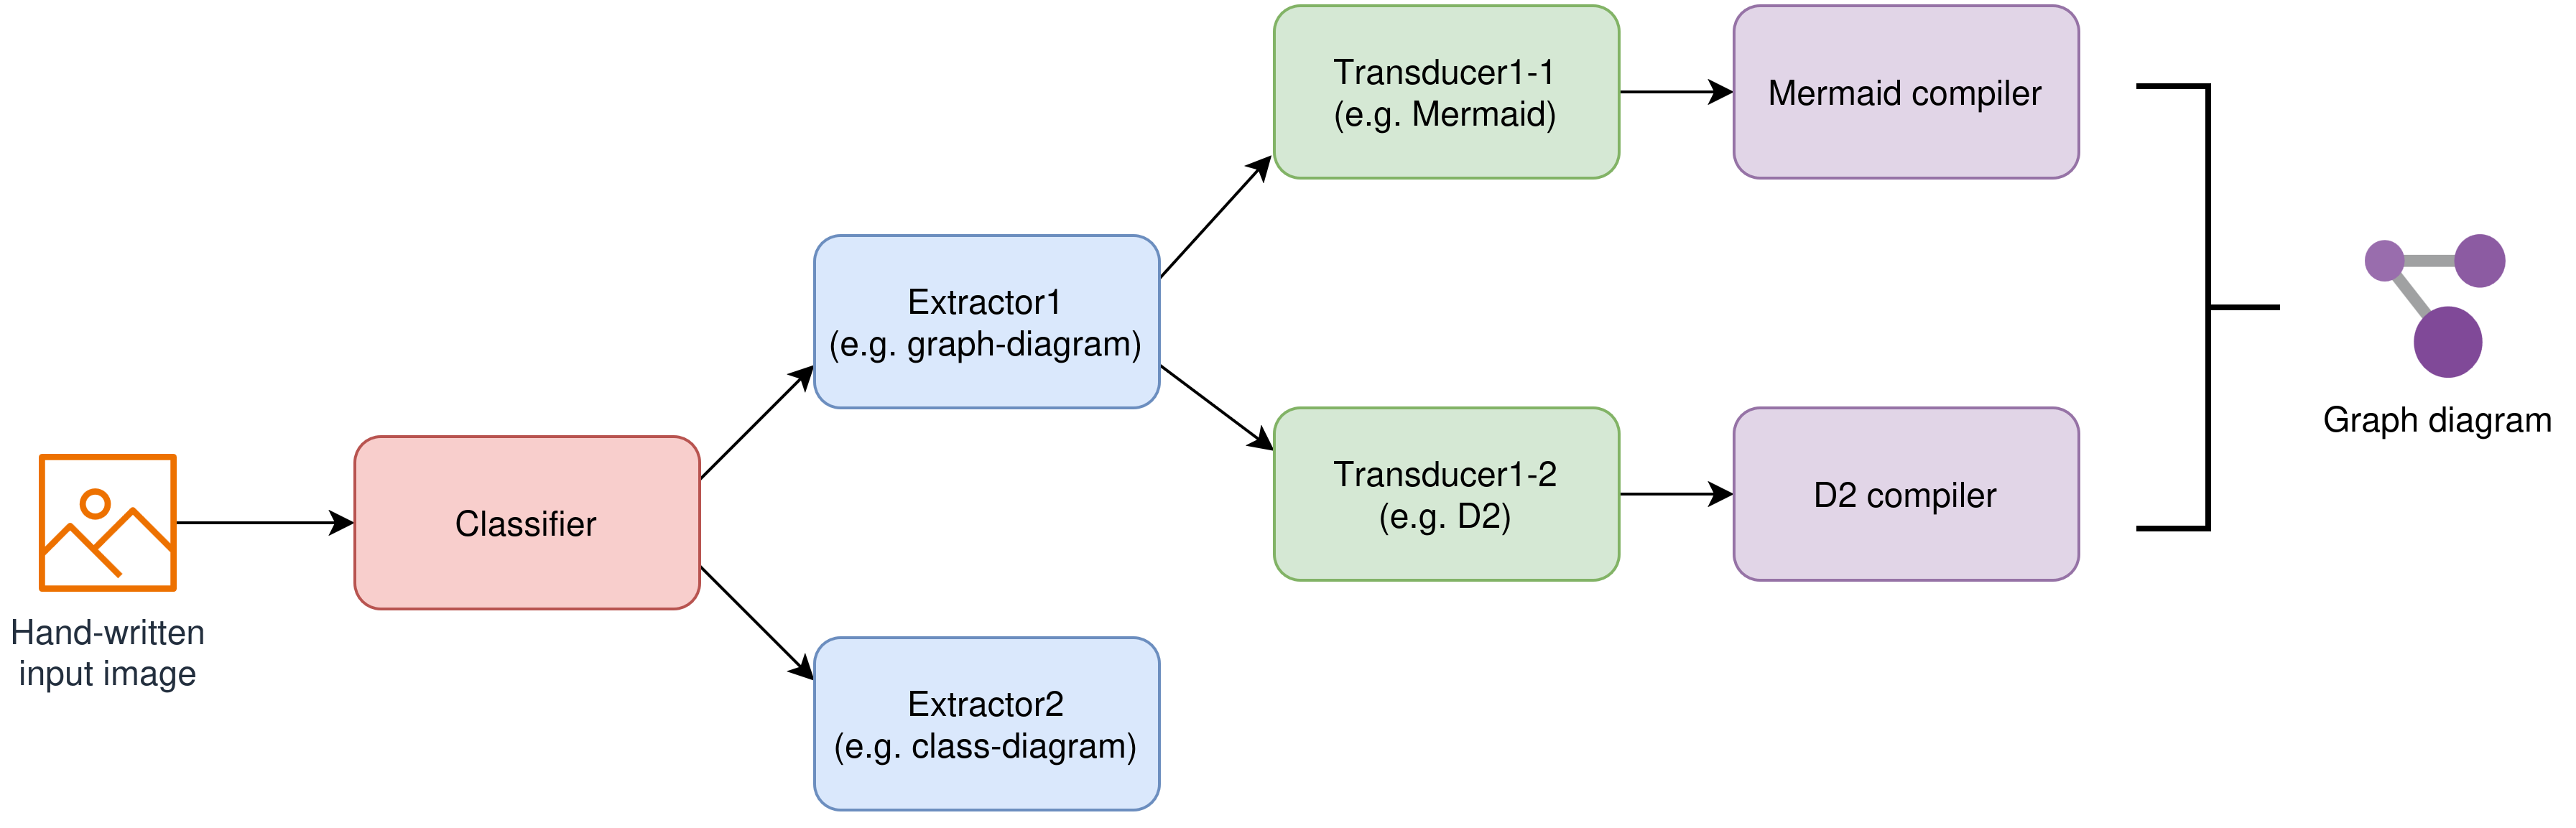
\includegraphics[width=\linewidth]{overview.png}
\caption{Overview of the D.I.A.G.R.A.M. system architecture.}
\label{fig:pipeline}
\end{figure}

The Classifier is able to recognize the category of the hand-written diagram that the user submitted as input. This is necessary in order for the system to know to which Extractor pass the data. This module is able to apply object detection and semantic recognition to represent the diagram in a unified way. After that, the representation is processed by the Transducer, which converts the data in a Markup language of choice. The Markup language content is therefore sent to the Compiler, thus generating the high-quality and editable diagram in PNG format.

\subsection{Classifier Module}
The Classifier is the first component of the pipeline. It is able to understand which category a given image of an handwritten diagram belongs to. This is necessary in order to later know the Extractors that can process the input image.
\subsection{Extractor Module}
The Extractor is the key component of the D.I.A.G.R.A.M. system, able to transform the raw diagram image into a structured, category-agnostic representation.
The Extractor recognizes the diagram's components, such as shapes, lines, and text, through an object detection network, and organizes them into a unified format. This representation serves as the foundation for the subsequent Transducer module, which converts the structured data into a domain-specific markup language.
\subsection{Transducer Module}
The Transducer is responsible for converting the unified, agnostic representation of a diagram into a domain-specific markup language. 
This transformation enables the subsequent Compiler module to generate high-quality visual outputs.
\subsection{Compiler Module}
The Compiler module is the final stage of the D.I.A.G.R.A.M. pipeline. 
Its primary role is to take the structured representation of the diagram, expressed in a markup language (e.g., \textit{Mermaid.js}), and generate a high-quality diagram in a visual format such as PNG. 

% 
% Flowchart Diagram
%
\section{Flowchart Diagram Recognition}

\subsection{Internal Representation}
In order to pass data through the components of the pipeline in a unified way, it was necessary to decide upon an internal representation of the flowchart diagram. It consists of \textbf{elements} and \textbf{relations}. The latter are linked to at least one element. Every element has a \textit{category} and possibly some \textit{inner} and \textit{outer text}. Every relation has a \textit{category} too, and could have a \textit{source} or \textit{target element}, and possibly \textit{text} related to it. The latter property is actually subdivided in four distinct boxes: the text could be associated with the arrow's head, tail, body or the text could be cut off by the arrow itself.

This internal representation is generated from the image provided by the user by the Extractor module, while it is parsed and converted to a markup language of choice by the Transducer. 

\subsection{Classifier Module}
\subsubsection{Preprocessing}
Due to the fact that various kinds of diagrams' images could be submitted to the system, it was decided to streamline a unified preprocessing pipeline in order to reduce the differences that our classifier model had to handle. A few problems were analyzed and the final preprocessing pipeline for the classifier module is composed of the following operators, in order:
\begin{itemize}
	\item \textbf{Gray Scaling}: In order to remove colors from images, which was deemed an useless information for classifying diagrams.
	\item \textbf{Otsu Thresholding}: To binarize the image and reducing the information to handle.
	\item \textbf{Median Filtering}: Some images in our dataset - and in the use-case - were taken on checkered notebooks. The application of a median filter, with kernel size equal to three, totally removed these.
	\item \textbf{Perspective Correction}: The diagrams' images, sometimes, didn't occupy the full photo frame. Finding four keypoints (if possible) and stretching the image helped to fully employ the frame.
	\item \textbf{Padding}: This was necessary in order to keep the same net for every image. Changes in resolution would have implied changes in the number of paramters of the MLP layers.
\end{itemize}

Figure~\ref{fig:classifier_preprocessing} shows the step-by-step process of preparing an input image for the network.

\begin{figure}[H]
	\centering
	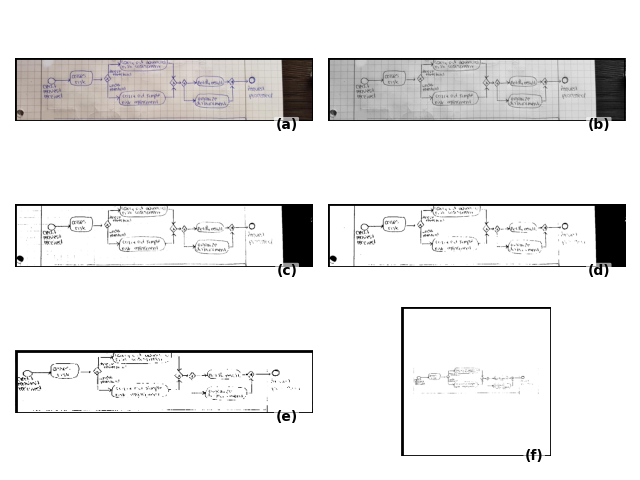
\includegraphics[width=220pt, height=150pt]{classifier_preprocessing.png}
	\caption{
		The operations applied by the preprocessing module.
		\textbf{(a)}: The raw image, still colored.
		\textbf{(b)}: The image in gray scale.
		\textbf{(c)}: The binarized image, thanks to Otsu.
		\textbf{(d)}: The median filter result. Some previous thin lines are now no more.
		\textbf{(e)}: The image with a perspective correction.
		\textbf{(f)}: The image in a standard size, ready to enter the network.
	}
	\label{fig:classifier_preprocessing}
\end{figure}


\subsubsection{Model}
Since it was assumed that classifying two types of diagrams - with a third 'other' class - was a quite simple task, a small network was deemed enough. The model consists of three convolutional blocks - each containing a convolutional layer, followed by a batch normalization and a max-pooling layer - then followed by three linear layers (for a more detailed overview, see Appendix~\ref{classification_net}). The output vector of the MLP contains three features - one for each class that this specific classifier needs to address. In order to determine the prediction, the softmax function is then applied. As later seen in section~\ref{exp:classifier}, a weighted Cross-Entropy loss is then used to train the model.

\subsection{Extractor Module}

The Extractor - despite its name - doesn't only need to \textit{extract} objects from images, but also to find connections. Its pipeline can be seen at \textbf{Figure} ~\ref{fig:flowchart-extractor}. \\

\begin{figure}
	\centering
	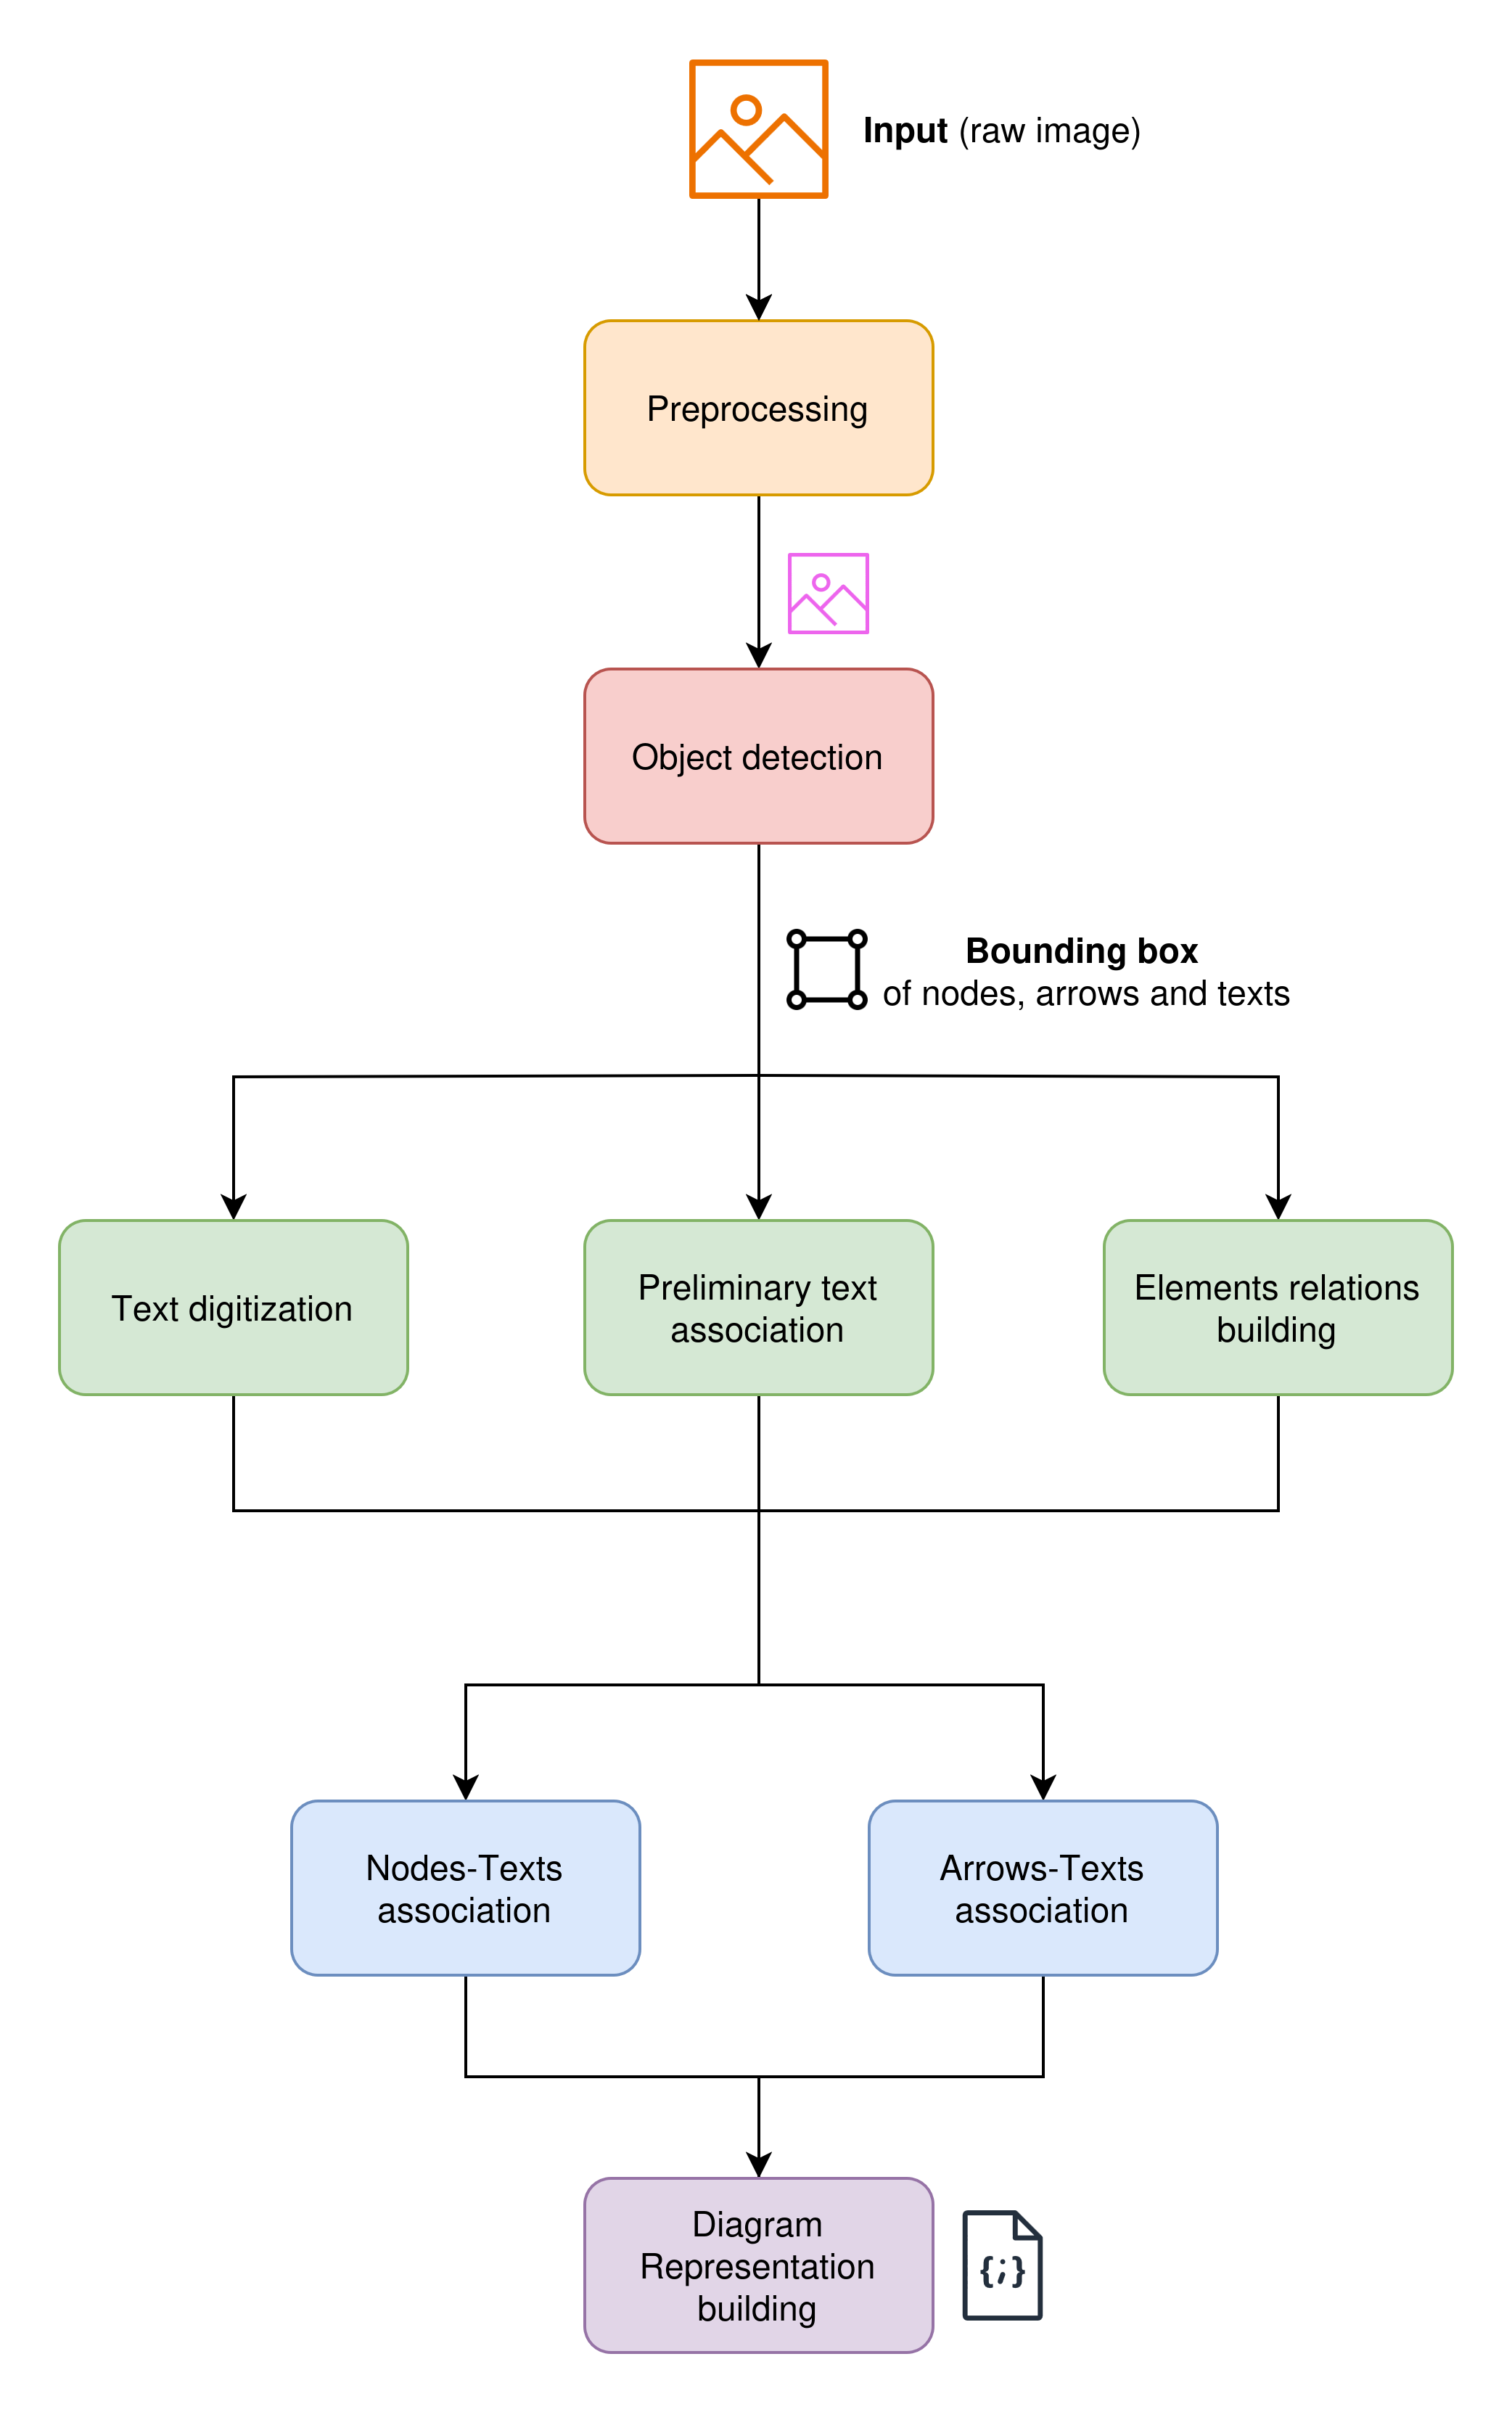
\includegraphics[width=\linewidth]{flowchart-extractor.png}
	\caption{The complete pipeline of the extractor module.}
	\label{fig:flowchart-extractor}
\end{figure}

\subsubsection{Preprocessing}
After some brief experiments, we found out that the object detection task through bounding boxes worked very well without any preprocessing technique. Moreover, the use of certain filters actually \textit{downgraded} the performances - e.g. the use of aggressive median filters reduced the capacity of the OCR model for text extraction.

The only preprocessing applied is a gray-scale transformation. Other transformations are not deemed necessary - the model employed automatically resize the input image, so it's not needed to do it beforehand. \\

\subsubsection{Bounding Box Detection}
\label{extr:bbd}
The model employed for object detection is a FasterRCNN, relying on a - as backbone - ResNet 50FPN~\cite{rcnn}. The image can be passed rough, and the model automatically resize the image to its own resolution. \\ 
After having determined all the bounding boxes of the diagram image, in order to correctly create the diagram internal representation, there's the need to link together text, elements and relations. For more details about the model and its training, refer to \textbf{Section}~\ref{sec:obj_det}. \\

\subsubsection{Arrow Retrieval}
Sometimes, the number of arrow's bodies, heads and tails don't match up. In particular, the following, trivial, equivalance doesn't hold true:
$$
	2\times\text{arrow bodies} = \text{arrow heads} + \text{arrow tails}
$$

The case in which, for a specific arrow, its head or its tail has not been found. In order to be able to be as error-robust as possible, we give the arrow - and a crop with more area around it - to the extraction net once again. If it's able to find both an head and a tail this time, we assume those to be the one's linked to the arrow. If more than one head or tail is found, the highest confidence result is kept - unless the confidence is lower than a certain threshold. 

The other case is the one in which we have some heads and tails without any body. For each pair of head and tail, the area of the image linking them is cropped and given to the detection net. For every arrow's bounding box found - if any - we compute the overlap with both the head and tail's bounding boxes. If the overlap is lower than a certain threshold, the arrow's bounding box is discarded. If it's over it and if it's over the current arrow's confidence value - if present, in the case in which we found multiple valid candidates - it's momentarily assumed as the correct arrow. If no arrow fulfills any of the above requisite, we discard the couple as candidates. \\

\begin{figure}[htbp]
	\centering
	
	% Row 1
	\begin{subfigure}[b]{0.45\linewidth}
		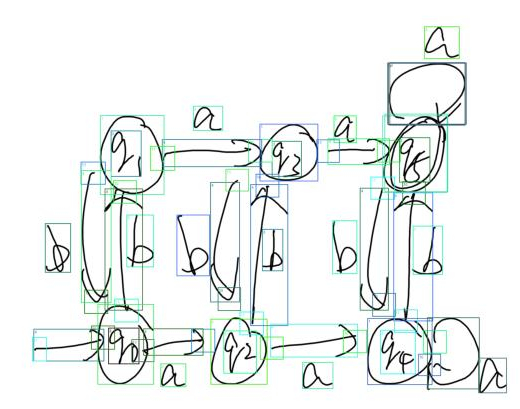
\includegraphics[width=\linewidth]{retrieval1.jpg}
		\caption{A graph diagram. The upper rightmost self-arrow has been detected - but not its tail and head.}
	\end{subfigure}
	\hfill
	\begin{subfigure}[b]{0.45\linewidth}
		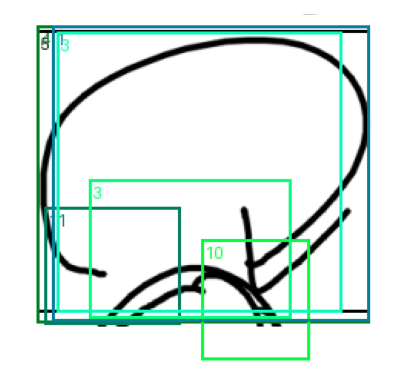
\includegraphics[width=\linewidth]{retrieval2.png}
		\caption{The detection net's output, able to recognize the arrow's head and tail after passing only a crop of the region.}
	\end{subfigure}
	
\end{figure}


\subsubsection{Arrow Orientation}
To later correctly assign arrows to their source and target elements, the need to determine where the tip of an arrow lies. This task involves a few problems, among which determining exactly the arrow shape and its end - because sometimes other pen signs may be found in the bounding box of the arrow itself. After a few trials (and errors; for further insight, refer to section~\ref{exp:arrow_orientation}), the approach yielding the best results was through the use of the object detection network (see section~\ref{extr:bbd}) to recognize both arrow heads and tails. \\

\subsubsection{Text Digitization}
Since the task of converting an image of text into the relative string has already been solved in various ways, we settled upon the Microsoft \textit{Trocr Handwritten} Transformer model; more precisely, the \textit{base} version of it \cite{microsofttrocr}. Every bounding box containing text that has been found is later passed to the model, and the resulting string generated by the model is linked to it.\\

\subsubsection{Relationships Building}
Once the text has been digitized, it's necessary to effectively compute which elements are connected by which arrows. This is done by finding, for each arrow, the elements nearer to the head (which we will assume to be the 'target' of the relation) and to the tail (the 'source' of the relationship exemplified by the arrow). These associations are nullified if the distance is above a certain adjustable threshold. This last step is done under the hypothesis that an arrow may come from nothing - or may point to nothing, having actually only either the source or the target. \\

\subsubsection{Text Association}
It can be assumed that every piece of text is linked to one and only one element or relation. So, every bounding box containing text is linked to the nearest element - it being either a relation or a node. The associations that require too long a distance are eliminated further in the algorithm, and the associated text is discarded.\\

\subsubsection{Node-Text Association}
After that a text box has been assigned to a node, there's the need to understand if the text is either inside or outside of the target node and whether the text is actually referring to the given element or not. In order to do this, the overlap between the two bounding boxes is computed; the value is compared to an heuristically determined threshold. If it's higher, the association is kept and the text is determined to be inside. If it's lower, the distance between the two bounding boxes is computed - as the distance between their central point. If the distance is below a certain threshold, the association is kept and the text is regarded as outside the node; otherwise, it's discarded.\\

\subsubsection{Arrow-Text Association}
After a text box is assigned to an arrow, some computation is needed to fully understand how the text is associated to the arrow itself. The arrow is approximated by a line adjoining its head and its tail.
The distance between the line and the text's bounding box is computed and compared with a threshold - if it's over it, the association is discarded.
Otherwise, the line approximation is then split into three different sections (see Figure~\ref{fig:arrowsplit}) - whose sizes are heuristically determined, such that the relation's central section is bigger than the other two. The distance between the text bounding box and each of the three sections boxes is computed - then, the section with the lowest distance value is then assigned to the text under consideration.
We must notice that for self-arrow we can not compute simple distance between the line and the text's bounding box, given that the approximated arrow line is not accurate. Thus, we approximate the arrow using two segments like a triangle.
The third point is the middle of the opposite edge (see Figure~\ref{fig:arrowapprox}). \\

\begin{figure}[H]
	\centering
	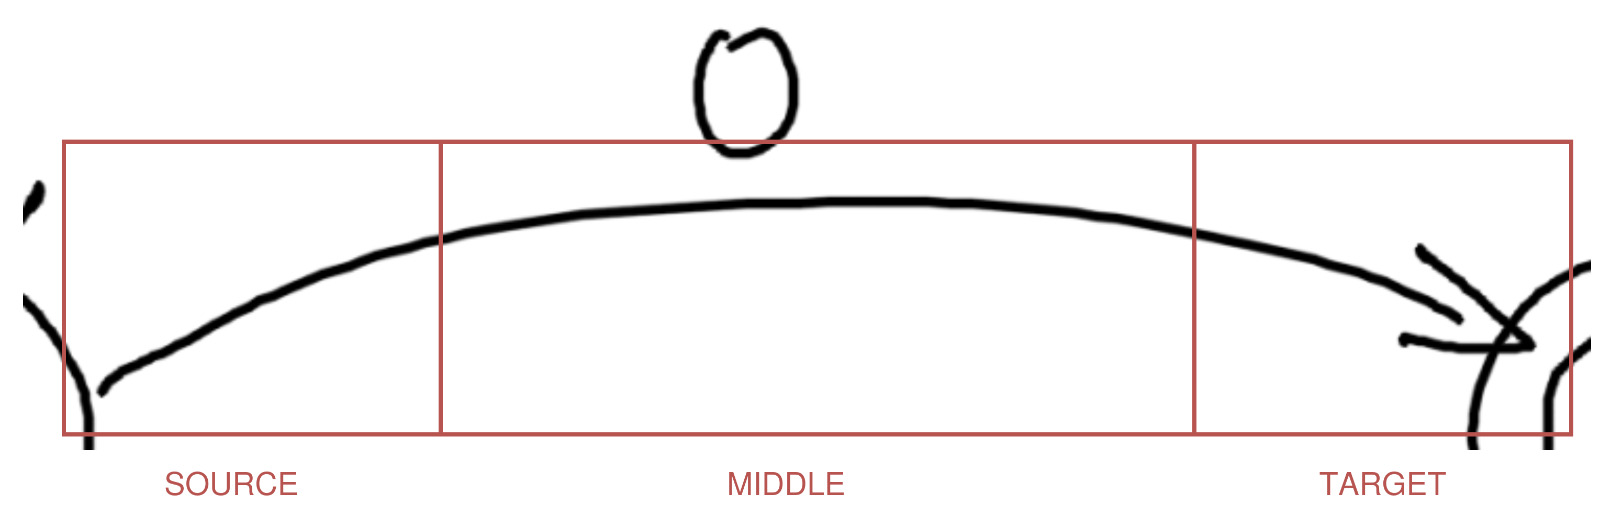
\includegraphics[width=\linewidth]{arrowsplit.jpg}
	\caption{A three-split of an arrow.}
	\label{fig:arrowsplit}
\end{figure}

\begin{figure}[H]
	\centering
	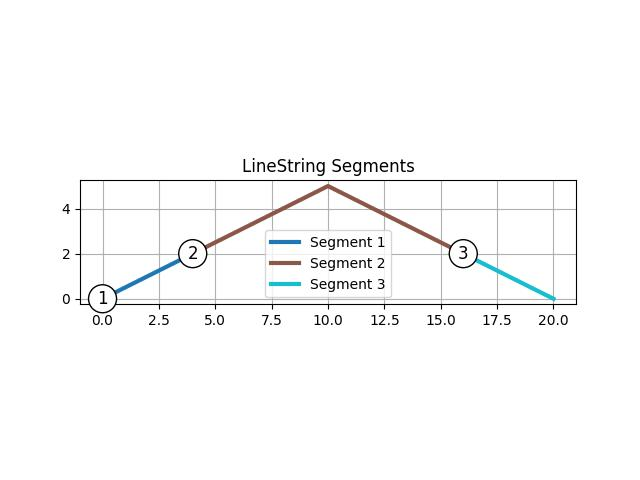
\includegraphics[width=\linewidth]{self_arrow.jpeg}
	\caption{Self-arrow approximation.}
	\label{fig:arrowapprox}
\end{figure}

\section{Dataset}
Our approach leverages multiple handwritten diagram datasets to ensure robustness across different diagram types and drawing styles. We employed a strategic dataset partitioning scheme where different subsets serve specific model training purposes.

\subsection{Dataset Sources}

We collected data from seven diverse sources, encompassing various diagram types commonly found in technical documentation and educational materials:

\begin{enumerate}
	\item \textbf{Finite Automata Dataset} \cite{online1}: Graph diagrams from the Czech Technical University collection, focusing exclusively on finite state machine representations.
	\item \textbf{Flowchart Dataset (FCB)} \cite{online3}: Flowchart diagrams from the Czech Technical University repository.
	\item \textbf{OHFCD\_1 Dataset} \cite{ohfcd}: Handwritten flowchart diagrams from the Computer Vision Center at UAB.
	\item \textbf{hdBPMN Dataset} \cite{BPMN}: Business Process Model and Notation diagrams from the Data and Web Science Lab.
	\item \textbf{Handwritten UML Class Diagrams} \cite{modelsketch}: Class diagram collection from Kaggle.
	\item \textbf{CircuitNet Dataset} \cite{circuitnet}: Electronic circuit diagram repository.
	\item \textbf{AI2D Dataset} \cite{ai2d}: Educational science diagrams from the Allen Institute for AI.
\end{enumerate}

Many datasets don't include the task at hand - which is focused on recognizing flowchart and graph diagrams - but could be in future works. Moreover, many datasets not apt to our task were used to further enhance the capability of the classifier - letting it know if an uploaded image couldn't be further processed.

\subsection{Dataset Usage Strategy}

We implemented a targeted approach for dataset utilization based on the specific requirements of our architecture:

\textbf{Classifier Training:} To enhance model robustness and generalization capabilities, we employed class diagrams, circuit diagrams, and school diagrams from the UML, CircuitNet, and AI2D datasets respectively. This diverse selection ensures the classifier can effectively distinguish between different diagram types across various domains.

\textbf{Extractor Training:} For the specialized extraction tasks, we focused exclusively on the first three datasets: flowchart and graph diagrams from the FCB, OHFCD\_1, and Finite Automata datasets. This targeted approach allows the extraction models to achieve high precision on the specific structural elements relevant to these diagram types, which were the core of our task. \\

\section{Experiments}

\subsection{Classifier}
\label{exp:classifier}
The first architecture explored for the Classifier module was a Convolutional Neural Network (CNN) following AlexNet's architecture \cite{alexnet}, but smaller in size.
It has two Convolutional layers, each followed by a batch normalization and then by a max pooling layers. The first layer had only 4 filters, while the second one had 8.
The output of the second layer was then flattened and passed through a fully connected layer which downsized the features to 128, followed by a ReLU activation function. Other two fully connected layer brought the number of output features down to the number of classes.
Then, a softmax activation function was applied to the output layer, in order to obtain the probabilities of each class.
The model was trained on our own dataset, with only three possible output classes: 'flowchart', 'graph' and 'other'; it was trained for 10 epochs, with an AdamW optimizer (with a learning rate of $0.001$) and a standard CrossEntropy Loss function. For a more comprehensive overview of the classifier's architecture, see Appendix~\ref{classification_net}.
\\

We first tried such a small network because the features that had to be recognized were very simple, down to the basic shapes of the diagram elements.
However, the results showed a non-decreasing value of the loss function of 0.9 - better than $-ln(3) \simeq 1.1$, which is random guessing, but still not satisfactory.
\\

Judging this to be a problem in architecture size, we then tried adding another CNN layer with 16 filters; this one too followed by a batch normalization and a max pooling layer.
The rest of the net was untouched; we also decreased the learning rate to $0.0001$, in order to avoid overshooting the minimum of the loss function.
The results, however, didn't show any kind of improvement, with the loss function still being around 0.9.
\\

While analyzing the predictions, we came up with what was actually the problem: the dataset was heavily unbalanced, with the 'other' class being the most represented one, shadowing the other two classes.
In order to solve this problem, we decided to use a weighted CrossEntropy Loss function, with the weights being inversely proportional to the number of samples in each class.

\begin{algorithm}
	\caption{Cross-Entropy weight computation}
	\begin{algorithmic}[1]
		\REQUIRE The classes' frequencies $f_1$, $f_2$, ..., $f_c$
		\STATE $S \gets \sum_{i = 1}^c f_i$
		\STATE $f_i \gets (f_i / S)^{-1}$
		\STATE $S \gets \sum_{i = 1}^c f_i$
		\STATE $f_i \gets f_i / S$
		\RETURN $f_1$, $f_2$, ..., $f_c$
	\end{algorithmic}
\end{algorithm}

This final approach showed a significant improvement in the results, with the loss function decreasing to around 0.6 after 10 epochs of training, with a global accuracy score of 97\% in the validation set.

\subsection{Object Detection}
\label{sec:obj_det}

For bounding box detection of diagram elements, we employed a Faster R-CNN architecture \cite{rcnn} with a ResNet-50 Feature Pyramid Network (FPN) backbone \cite{lin2017feature}. This two-stage object detection framework provides robust performance for multi-class detection tasks while maintaining computational efficiency suitable for diagram analysis applications.
Its main components are:

\textbf{Backbone Network:} The ResNet-50 backbone serves as the feature extraction component, providing representations through its four residual blocks.

\textbf{Feature Pyramid Network:} The FPN enhancement augments the ResNet-50 backbone features by creating a top-down pathway with connections.

\textbf{Region Proposal Network (RPN):} The RPN generates object proposals by sliding a small network over the feature maps from the FPN. At each spatial location, the RPN predicts object presence probability and bounding box refinements for different scales and aspect ratios.

\textbf{ROI Head:} The second stage performs precise classification and bounding box regression on the proposals generated by the RPN. Feature vectors are extracted using ROI Align operations. \\

The original model was trained over the COCO dataset \cite{coco}, which comprised 91 classes. It should be highlighted that the original training dataset was not in any way related to diagrams: with an efficient finetune, the network was able to swiftly change to our task. The finetuning is done with a learning rate of $0.005$ \\

The model employed was tested in three different ways: as zero-shot, after a 10-epoch training and after a 100-epoch training. The best-behaving one was, of course, the latter (to see the results of the different stages, see \textbf{Figures}~\ref{fig:bbox1} -~\ref{fig:bbox3} -~\ref{fig:fc}). In Table~\ref{tab:map} and Table~\ref{tab:mar} we show the Mean Average Precision and Recall of the model used.

\begin{figure}[H]
	\centering
	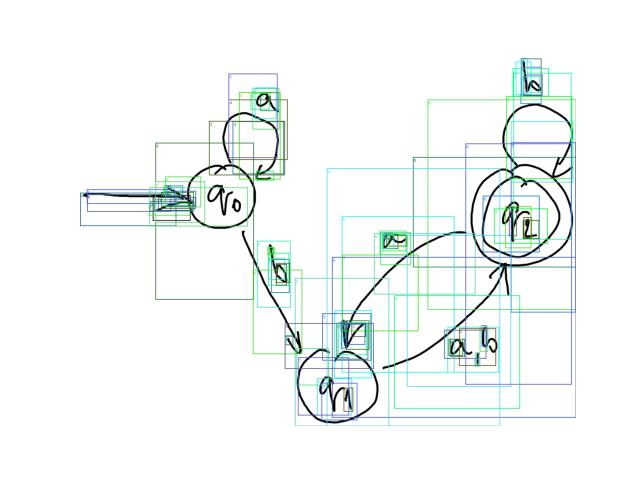
\includegraphics[width=200pt, height=150pt]{bbox1.jpg}
	\caption{The model employed in a zero-shot fashion.}
	\label{fig:bbox1}
\end{figure}

\begin{figure}[H]
	\centering
	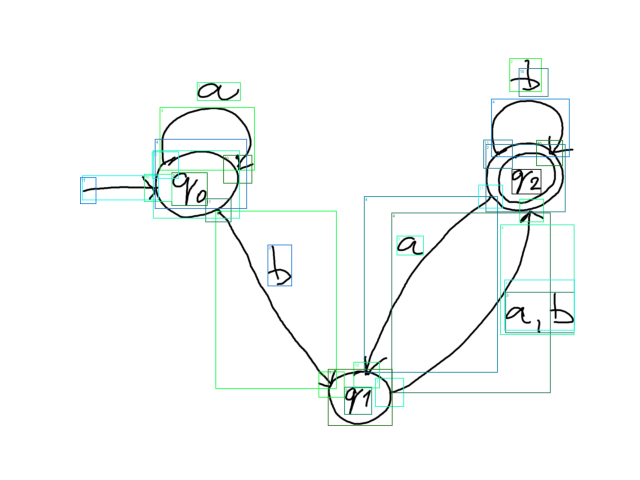
\includegraphics[width=180pt, height=150pt]{bbox3.png}
	\caption{The model employed after 100 epochs of training. With respect to Figure~\ref{fig:bbox1}, we also added here the heads and the tails for the arrows.}
	\label{fig:bbox3}
\end{figure}

\begin{figure}[H]
	\centering
	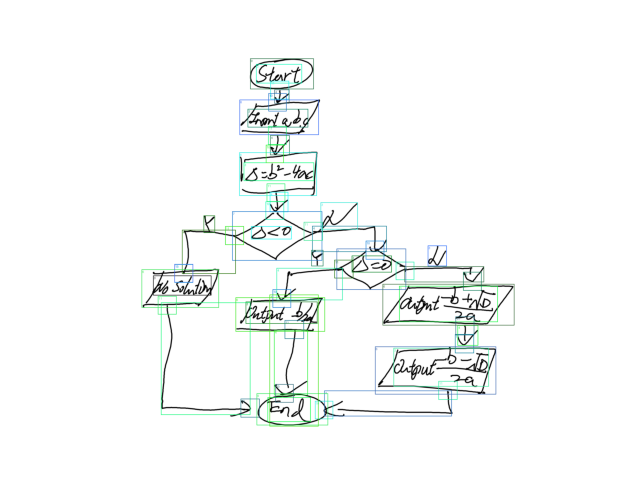
\includegraphics[width=180pt, height=150pt]{fc.png}
	\caption{The bounding boxes of a flowchart diagram, on the 100-epoch model.}
	\label{fig:fc}
\end{figure}

\begin{table}[htbp]
	\centering
	\caption{Mean Average Precision (\textit{mAP}) Metrics}
	\begin{tabular}{|l|c|l|}
		\hline
		\textbf{Metric} & \textbf{Value} & \textbf{Description} \\
		\hline
		mAP & 0.8754 & Overall mean Average Precision \\
		mAP@0.5 & 0.9878 & mAP at IoU threshold 0.5 \\
		mAP@0.75 & 0.9183 & mAP at IoU threshold 0.75 \\
		\hline
		mAP (Small) & 0.6444 & mAP for small objects \\
		mAP (Medium) & 0.8054 & mAP for medium objects \\
		mAP (Large) & 0.8975 & mAP for large objects \\
		\hline
	\end{tabular}
	\label{tab:map}
\end{table}

\begin{table}[htbp]
	\centering
	\caption{Mean Average Recall (\textit{mAR}) Metrics}
	\label{tab:mar}
	\begin{tabular}{|l|c|l|}
		\hline
		\textbf{Metric} & \textbf{Value} & \textbf{Description} \\
		\hline
		mAR@1 & 0.3436 & mAR with max 1 detection per image \\
		mAR@10 & 0.8877 & mAR with max 10 detections per image \\
		mAR@100 & 0.9128 & mAR with max 100 detections per image \\
		\hline
		mAR (Small) & 0.6631 & mAR for small objects \\
		mAR (Medium) & 0.8670 & mAR for medium objects \\
		mAR (Large) & 0.9141 & mAR for large objects \\
		\hline
	\end{tabular}
\end{table}

Furthermore, we also think that the following metrics show a great precision:

\begin{itemize}
	\item \textbf{Average X-axis error:} 6.84 pixels
	\item \textbf{Average Y-axis error:} 4.84 pixels
\end{itemize}


\subsection{Arrow Orientation}
\label{exp:arrow_orientation}
As we've seen in the previous section, the need to find the exact position of an arrow's head arises (see \textbf{Appendix~\ref{double_clustering} and \textbf{Appendix}~\ref{arrow-net}} for a full overview of the first approaches).

The solution, as stated before, was to finetune the already working Faster R-CNN in order for it to also extract the bounding boxes of both tails and heads of the arrow.

\subsection{Text Digitization}
In order to choose an appropriate model, some tests were done over our specific dataset employing some different, pre-made models. The average results over the dataset are shown in Table~\ref{tab:text_digitization}.

\begin{table}[htbp]
\caption{Text Distance Metrics}
\centering
\begin{tabular}{lccc}
\hline
\textbf{Model} & \textbf{Hamming} & \textbf{Cosine} & \textbf{Euclidean} \\
\hline
microsoft-trocr-small-printed & 1.392 & 0.150 & 7133 \\
% microsoft-trocr-base-printed & 1.286 & 0.081 & 3594 \\
microsoft-trocr-small-handwritten & \textbf{1.346} & 0.100  & 3947 \\ 
\hline 
\textbf{microsoft-trocr-base-handwritten} & 1.549 & \textbf{0.057} & \textbf{3003} \\
\hline
\end{tabular}
\label{tab:text_digitization}
\end{table}

Some examples of the different models applied to our flowchart diagram dataset can be seen in Figure~\ref{fig:text_digitization_results_1} and in Figure~\ref{fig:text_digitization_results_2}. \\

\begin{figure}[H]
\centering
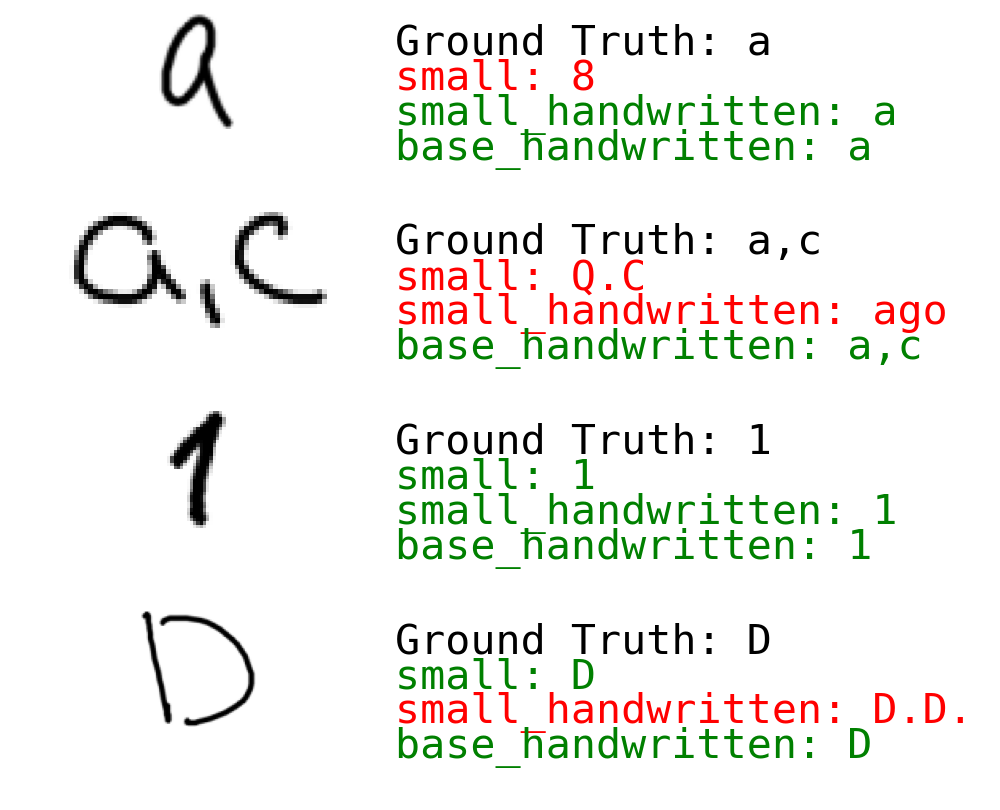
\includegraphics[width=\linewidth]{text_digitization_results_1.png}
\caption{Some random results of the text digitization over the proposed models.}
\label{fig:text_digitization_results_1}
\end{figure}

\begin{figure}[H]
\centering
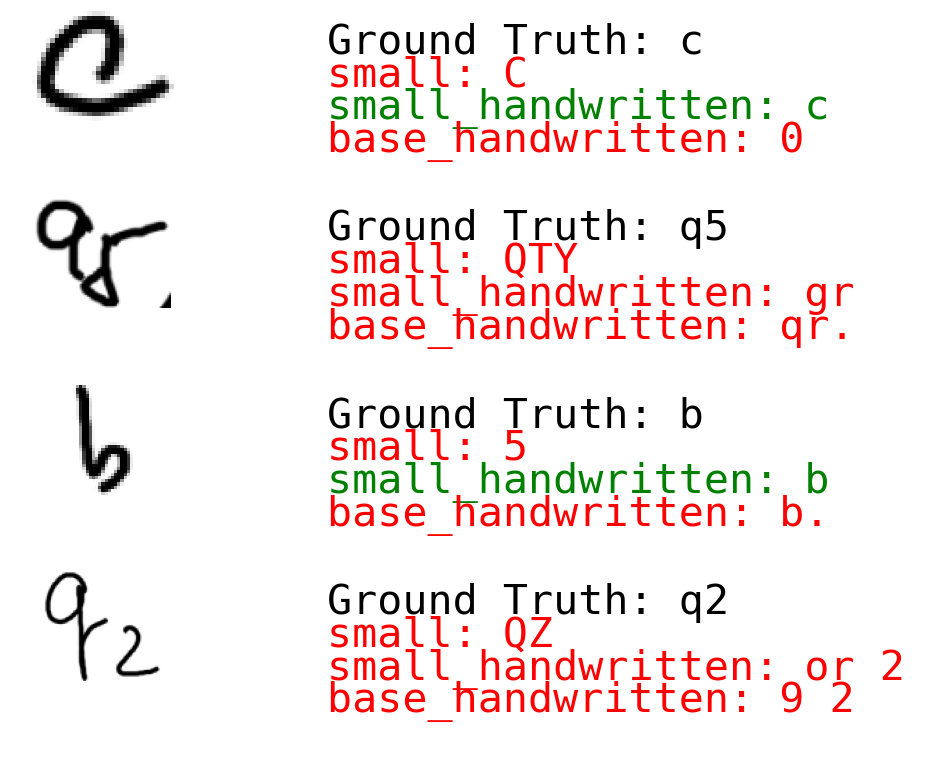
\includegraphics[width=\linewidth]{text_digitization_results_2.png}
\caption{Some results in which the \textit{trocr-base-handwritten} fails.}
\label{fig:text_digitization_results_2}
\end{figure}

\section{Discussion}

The development of D.I.A.G.R.A.M. offers an insightful perspective on the integration of deterministic logic and deep learning for the interpretation of handwritten diagrams. One of the most valuable outcomes of this project is the successful design of a complete and functional pipeline (see Figure~\ref{fig:results}), which transforms raw visual input into a structured, editable format. This end-to-end workflow—from classification to rendering—highlights the feasibility of modular architectures for diagram understanding.

\begin{figure}[htbp]
	\centering
	
	% Row 1
	\begin{subfigure}[b]{0.45\linewidth}
		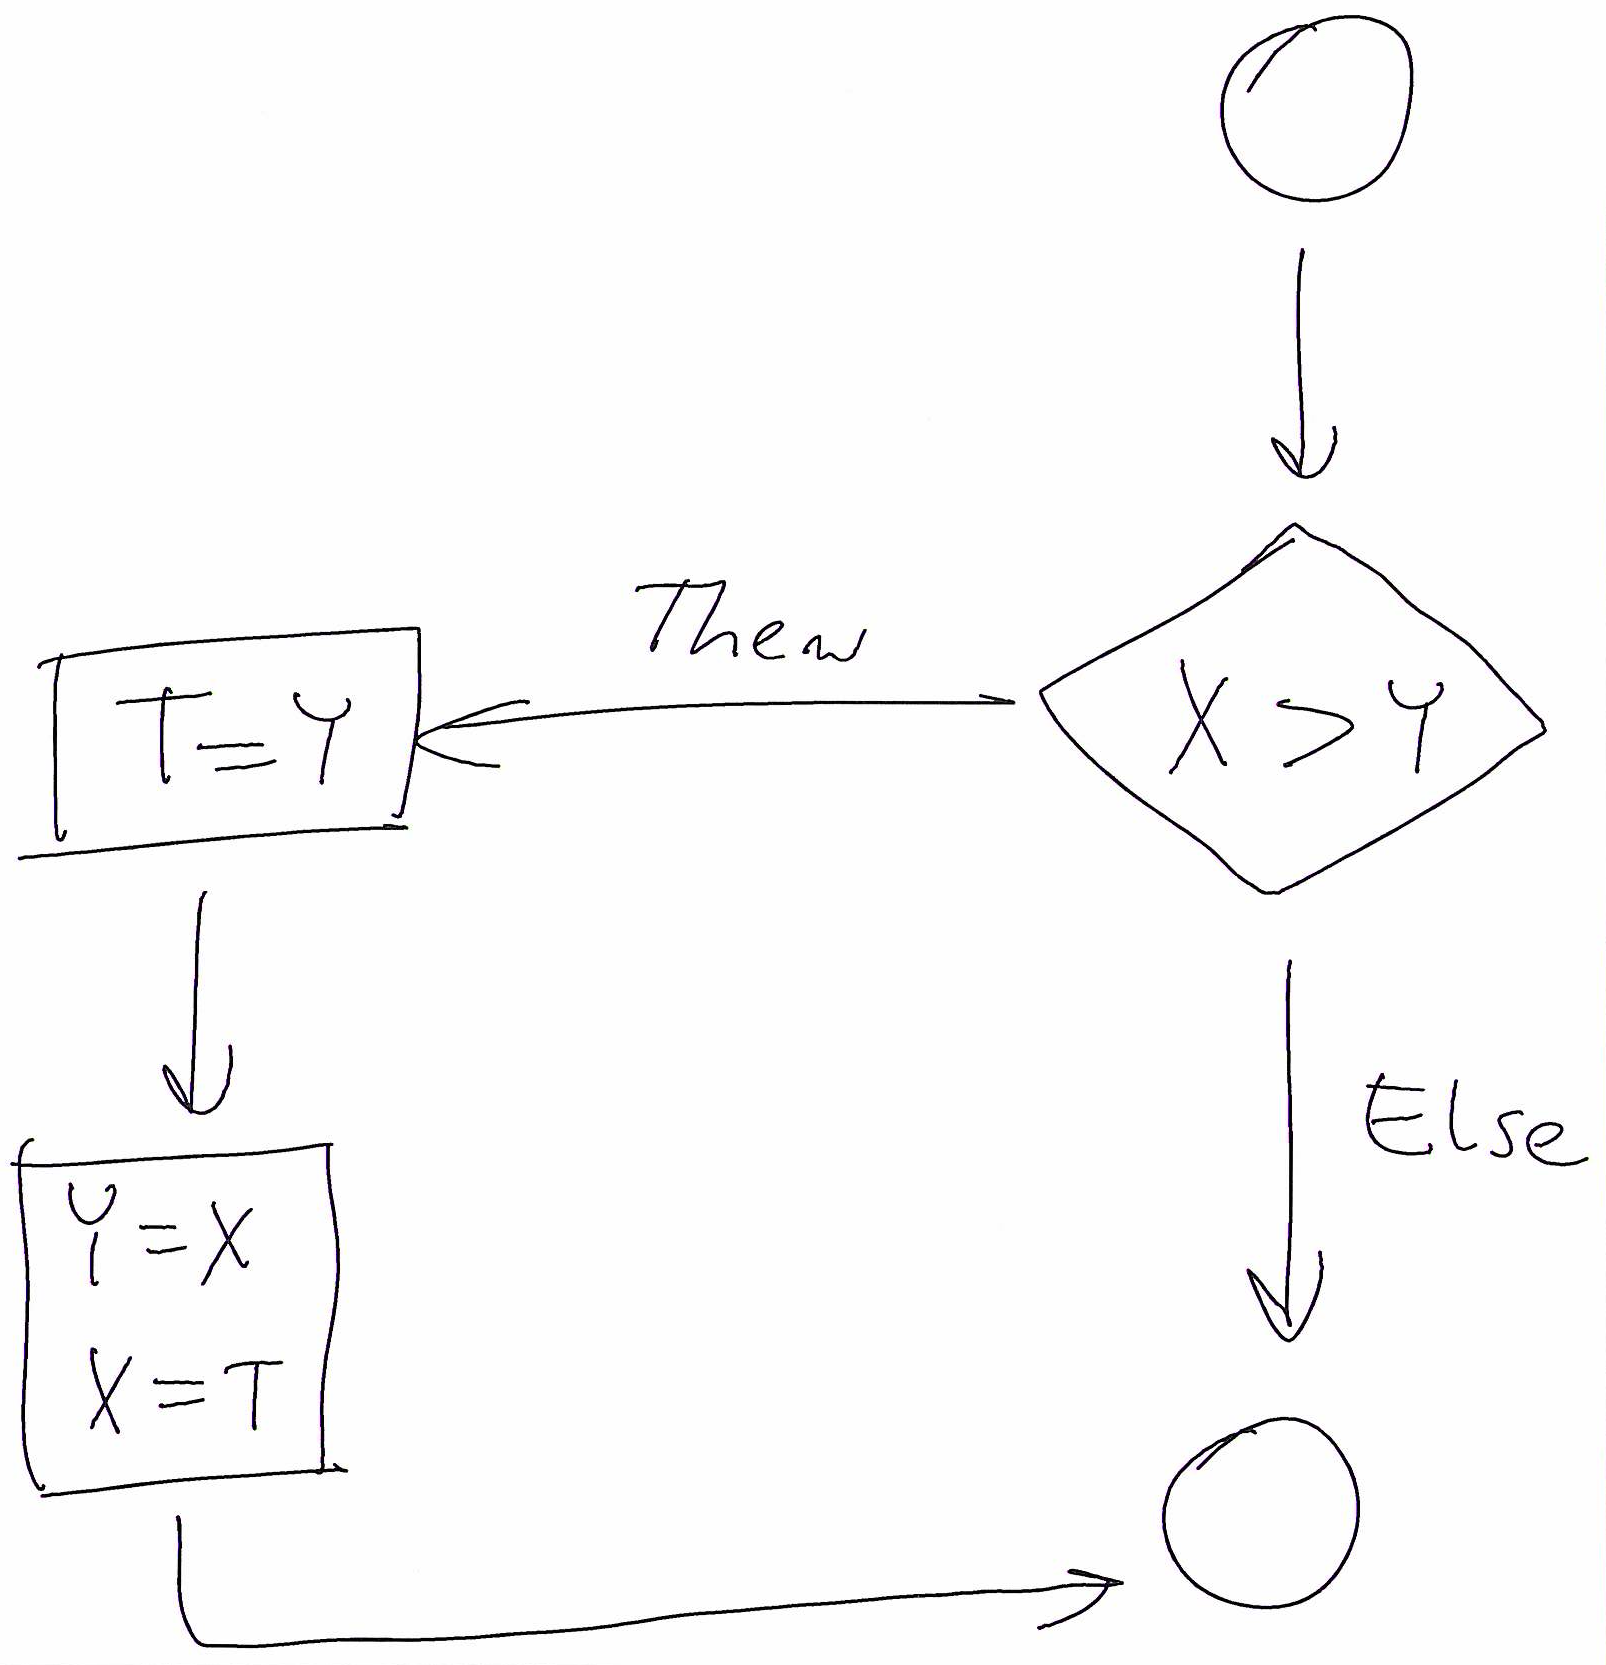
\includegraphics[width=\linewidth]{ex1.png}
		\caption{An easy flowchart diagram.}
	\end{subfigure}
	\hfill
	\begin{subfigure}[b]{0.45\linewidth}
		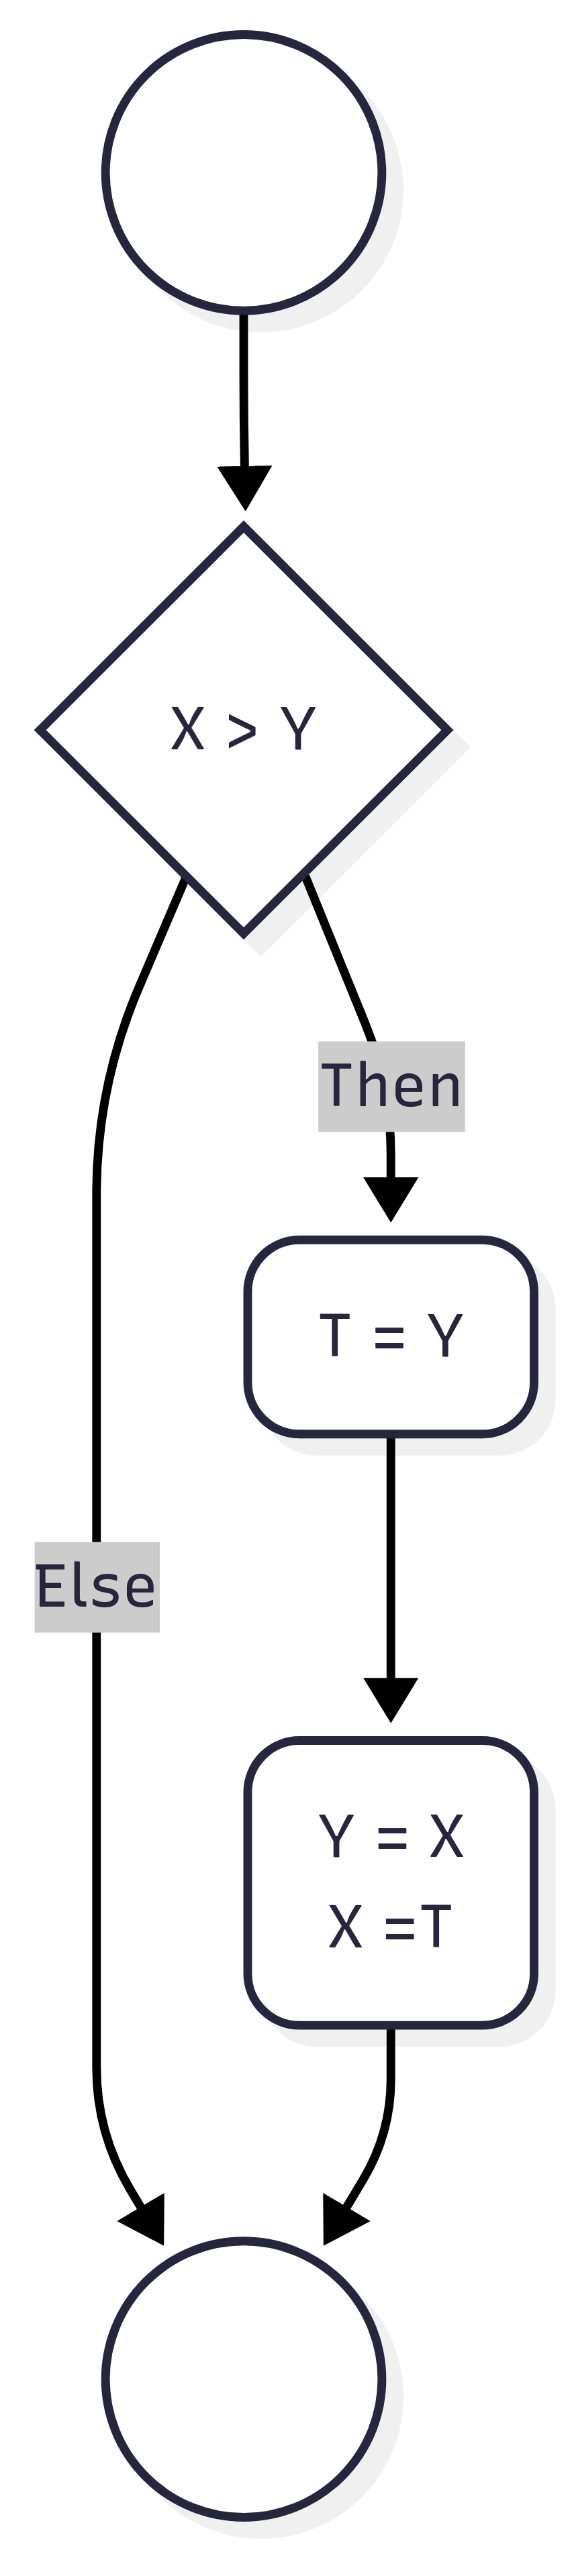
\includegraphics[width=35pt, height=150pt]{ex2.png}
		\caption{The network's output.}
	\end{subfigure}
	
	\vspace{1em} % spacing between rows
	
	% Row 2
	\begin{subfigure}[b]{0.45\linewidth}
		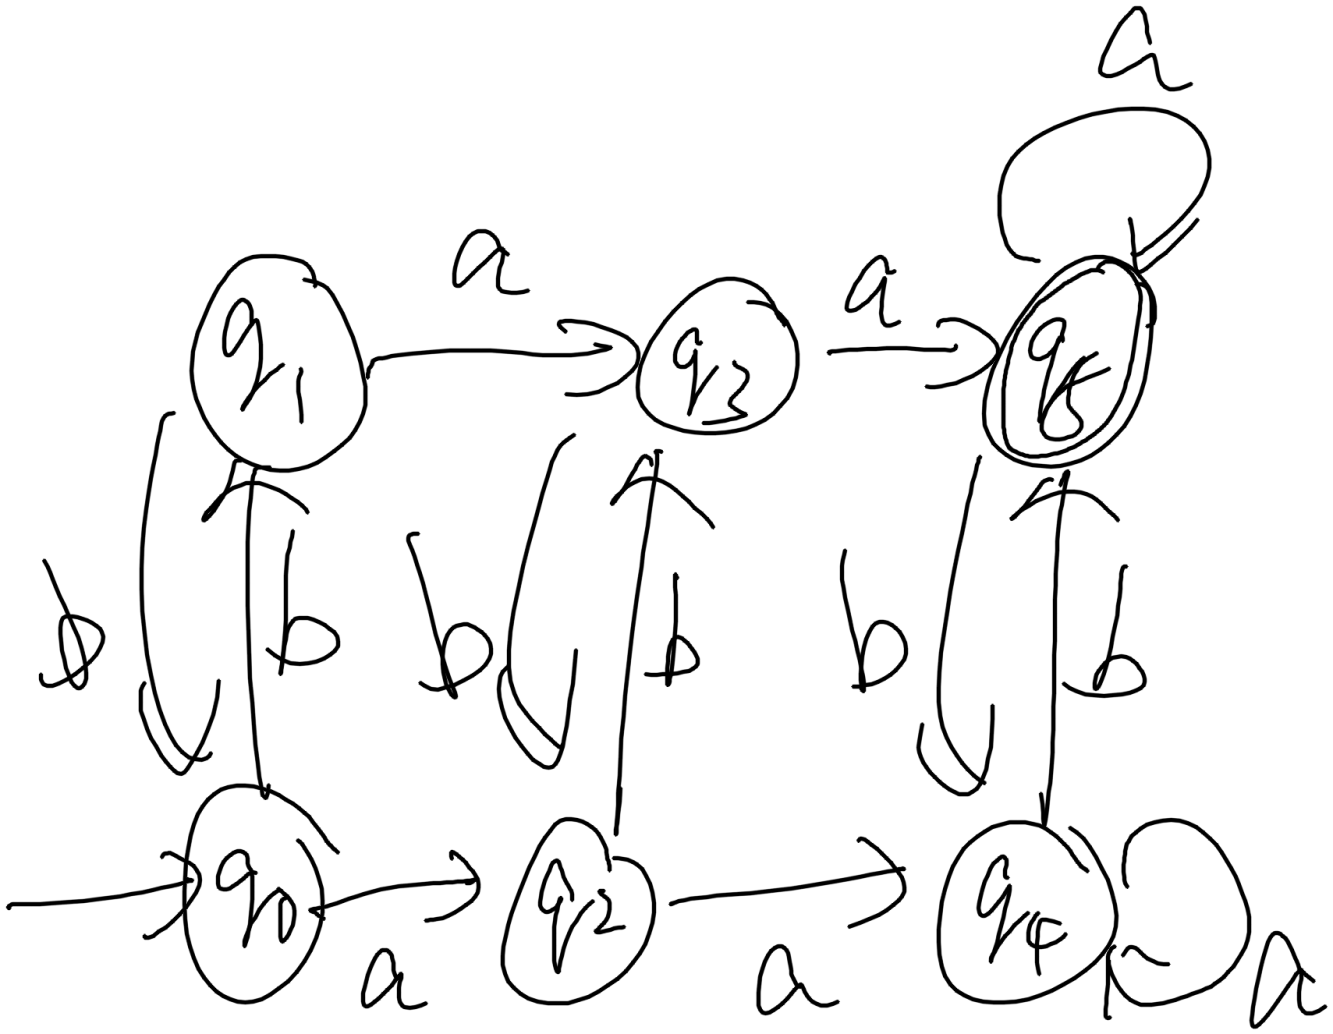
\includegraphics[width=\linewidth]{ex3.png}
		\caption{A complex graph diagram.}
	\end{subfigure}
	\hfill
	\begin{subfigure}[b]{0.45\linewidth}
		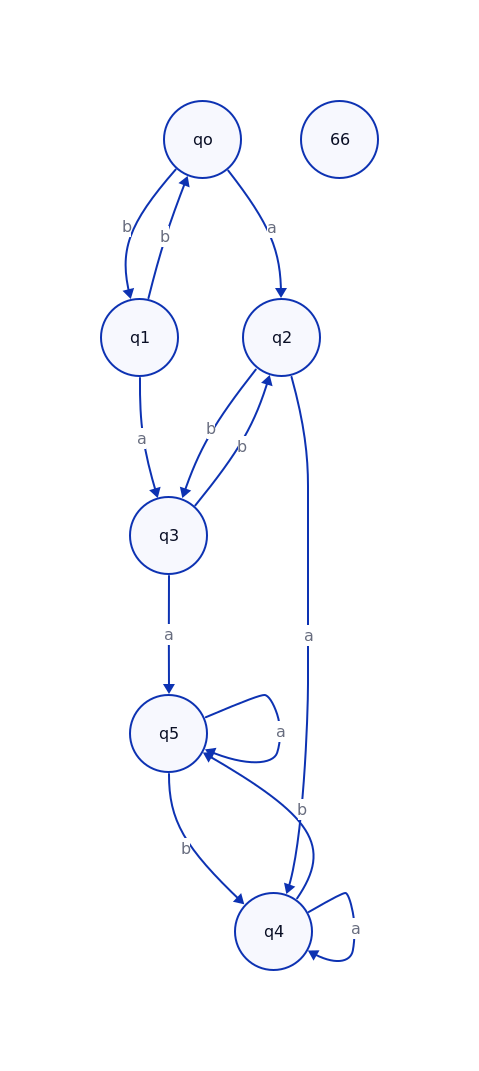
\includegraphics[width=50pt, height=130pt]{ex4.png}
		\caption{The network's output.}
	\end{subfigure}
	
	\vspace{1em}
	
	% Row 3
	\begin{subfigure}[b]{0.45\linewidth}
		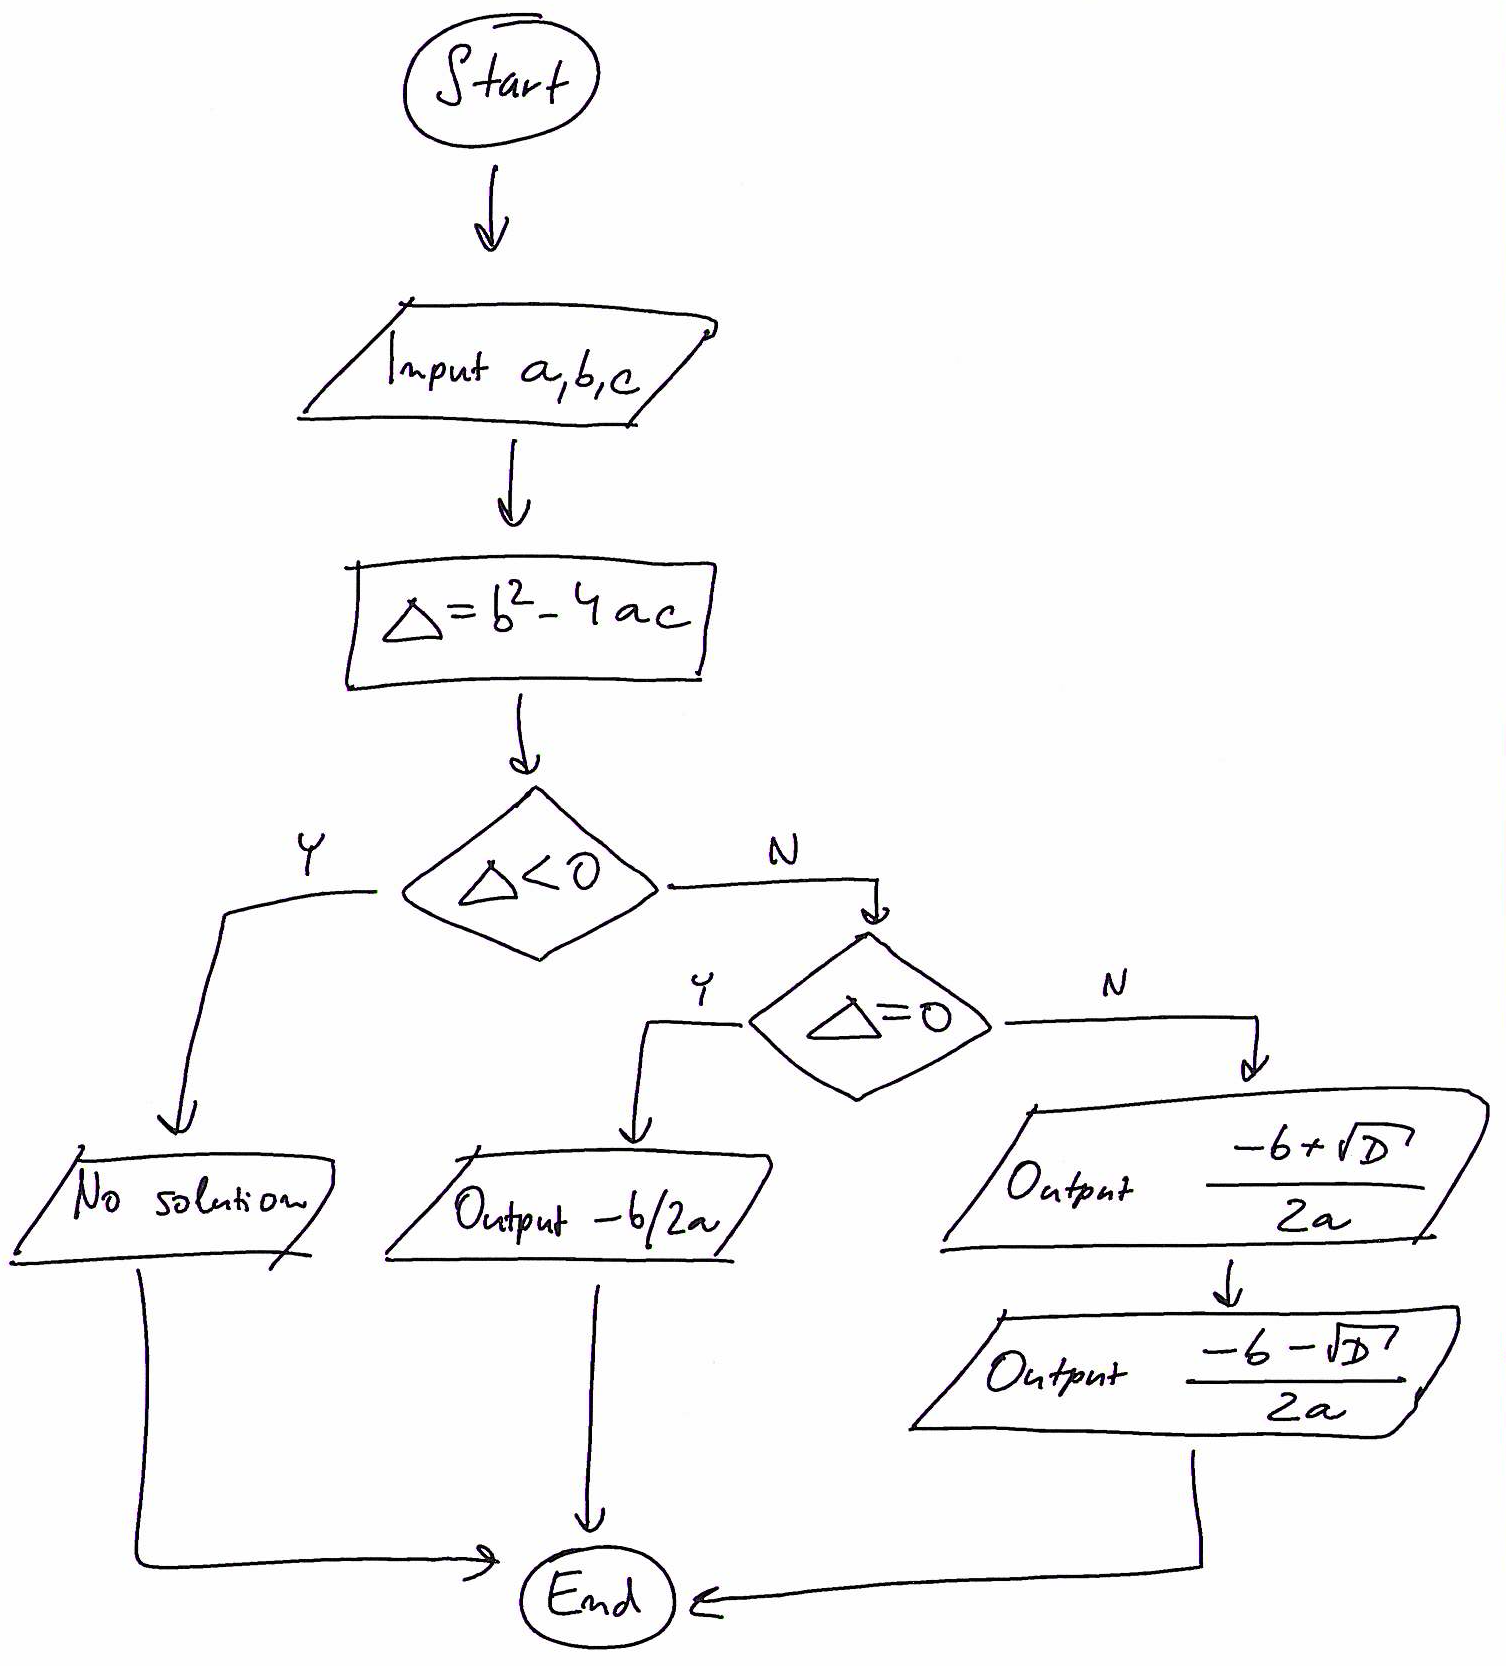
\includegraphics[width=\linewidth]{ex5.png}
		\caption{A complex flowchart diagram.}
	\end{subfigure}
	\hfill
	\begin{subfigure}[b]{0.45\linewidth}
		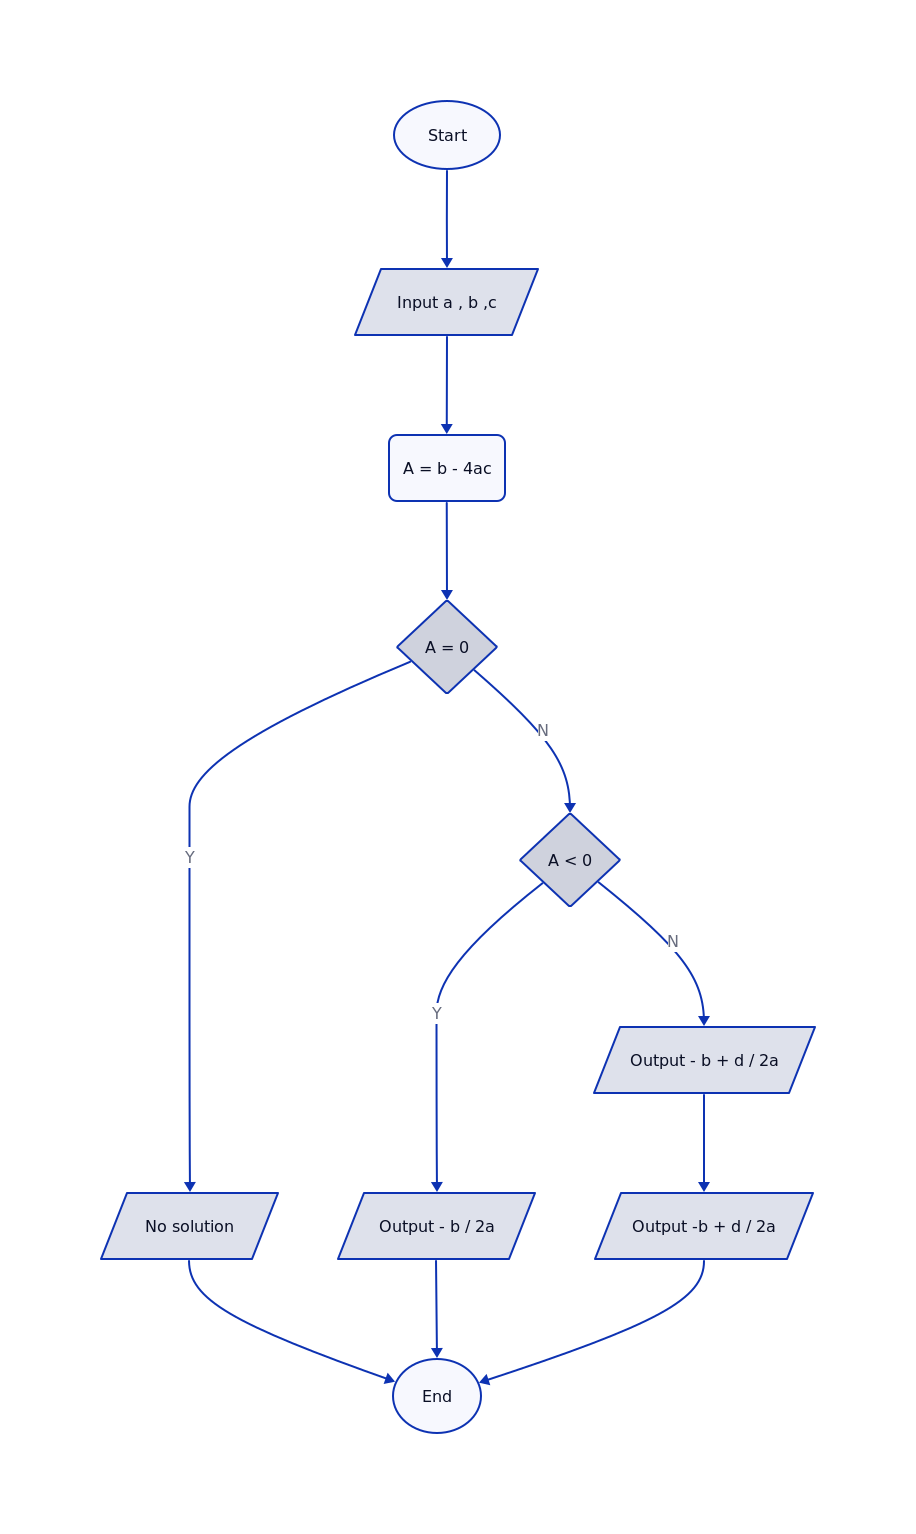
\includegraphics[width=70pt, height=130pt]{ex6.png}
		\caption{The network's output.}
	\end{subfigure}
	
	\caption{A few results of our network.}
	\label{fig:results}
\end{figure}

Among the modules, the Extractor proved particularly effective. Leveraging deep neural networks, it reliably identified diagram elements across diverse samples, validating the suitability of data-driven approaches for this subtask. Conversely, the Classifier, while operational, showed room for improvement, particularly in edge cases or less represented diagram categories. This suggests that the current training set may lack the diversity required for robust generalization, pointing to data augmentation and dataset expansion as immediate avenues for refinement.

The system as a whole adheres to principles of scalability and generality. By decoupling the diagram type detection from the extraction and compilation logic, D.I.A.G.R.A.M. maintains flexibility in handling new diagram formats with minimal architectural changes. However, its performance remains sensitive to input quality and assumes a level of neatness in the handwritten diagrams that may not always be guaranteed in real-world scenarios.

In comparison to related work, D.I.A.G.R.A.M. distinguishes itself by targeting offline, image-based recognition (as opposed to stroke-based online methods) while retaining support for structural output generation. This positions it as a hybrid between traditional rule-based recognizers and modern neural approaches. \\

We'd like to point out a few things about the results shown Figure~\ref{fig:results}. First of all, the result shown in part (d). A non-existing node can be seen in the upper right corner of the image; this is due to the fact that the self-arrow of node $q_5$ is recognized - by the object detection network - both as an arrow and as a node, with an high trust value. This problem could have been solved by applying a Non-Maxima Suppression - but in this specific case, the highest confidence value was surprisingly the node's one. This problem - that occasionally shows up - is probably to be attributed to the low samples present in the dataset.

\begin{figure}[h!]
	\centering
	\vspace{0.5em}
	
	% First row
	\begin{tabular}{ccc}
		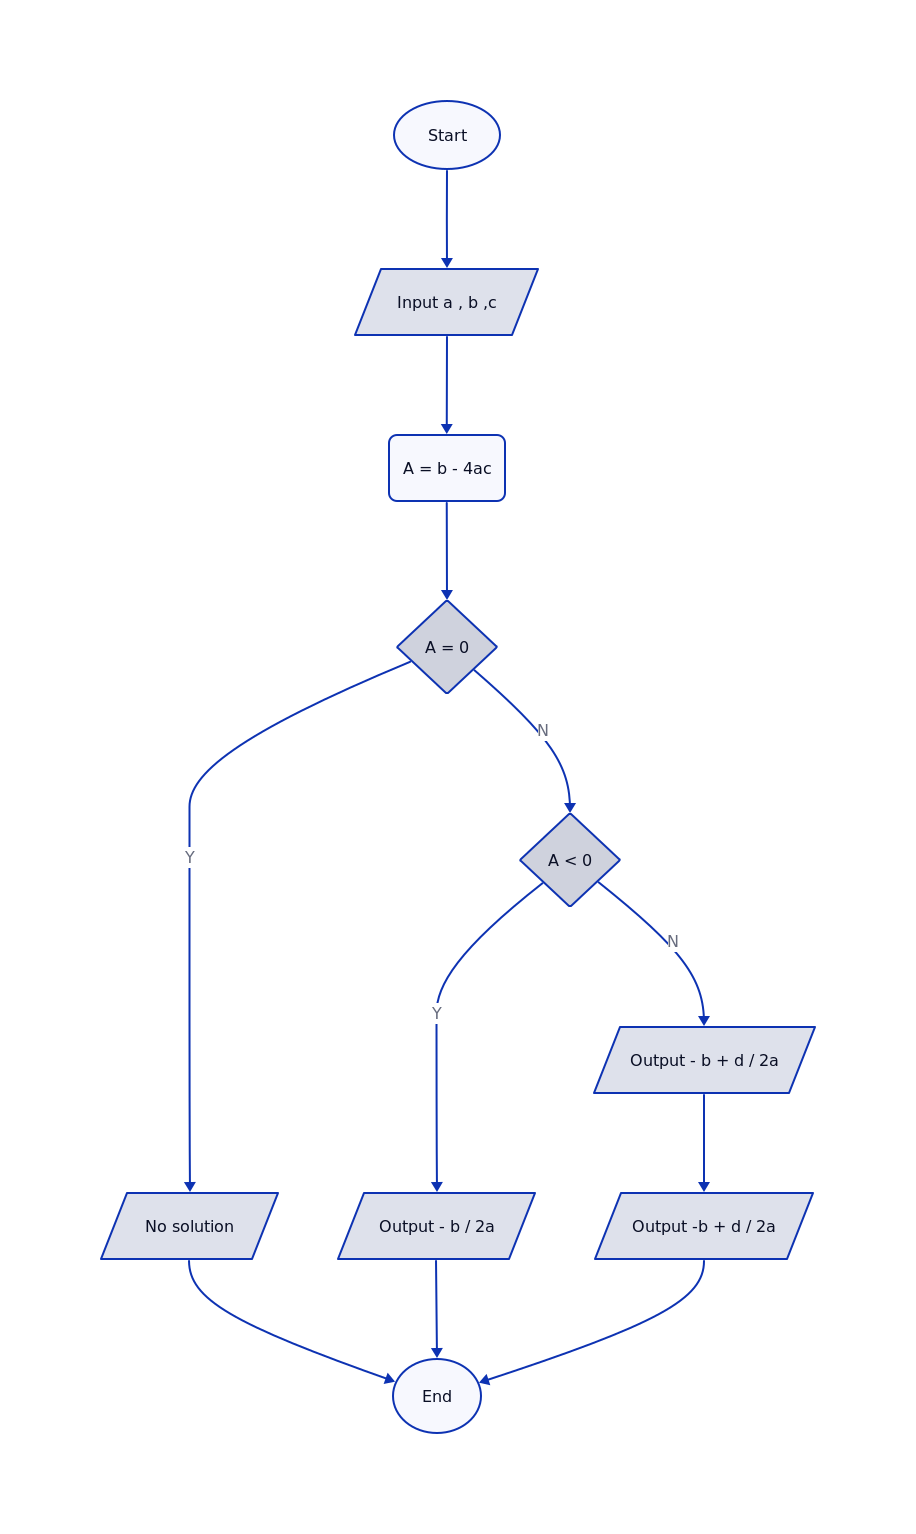
\includegraphics[height=5cm]{ex6.png} &
		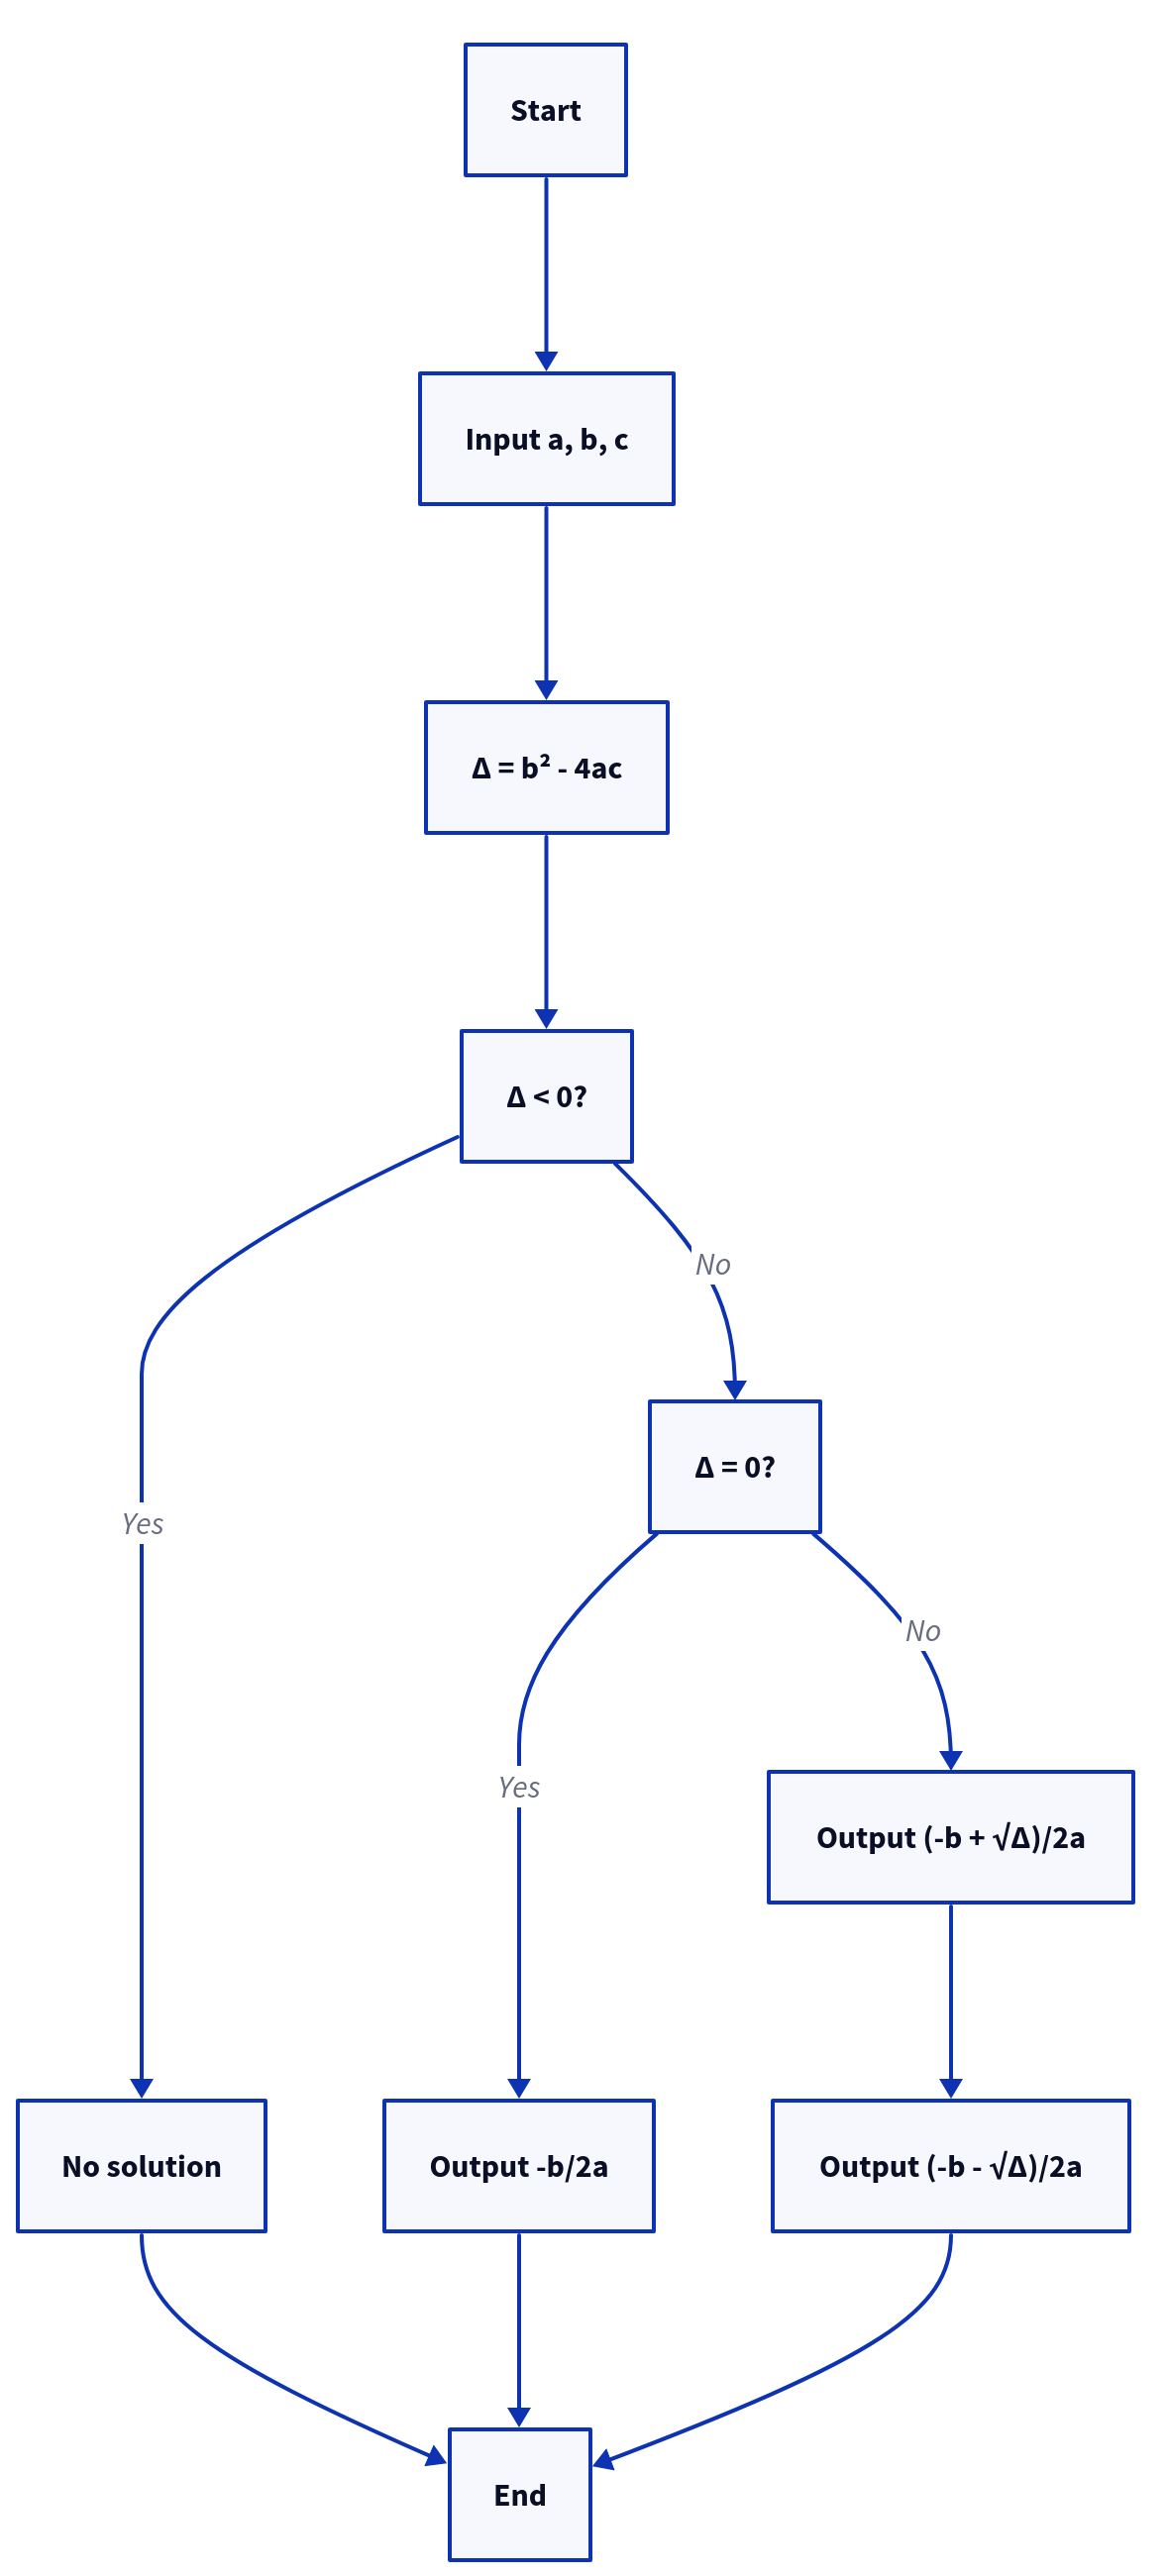
\includegraphics[height=5cm]{chat1.png} &
		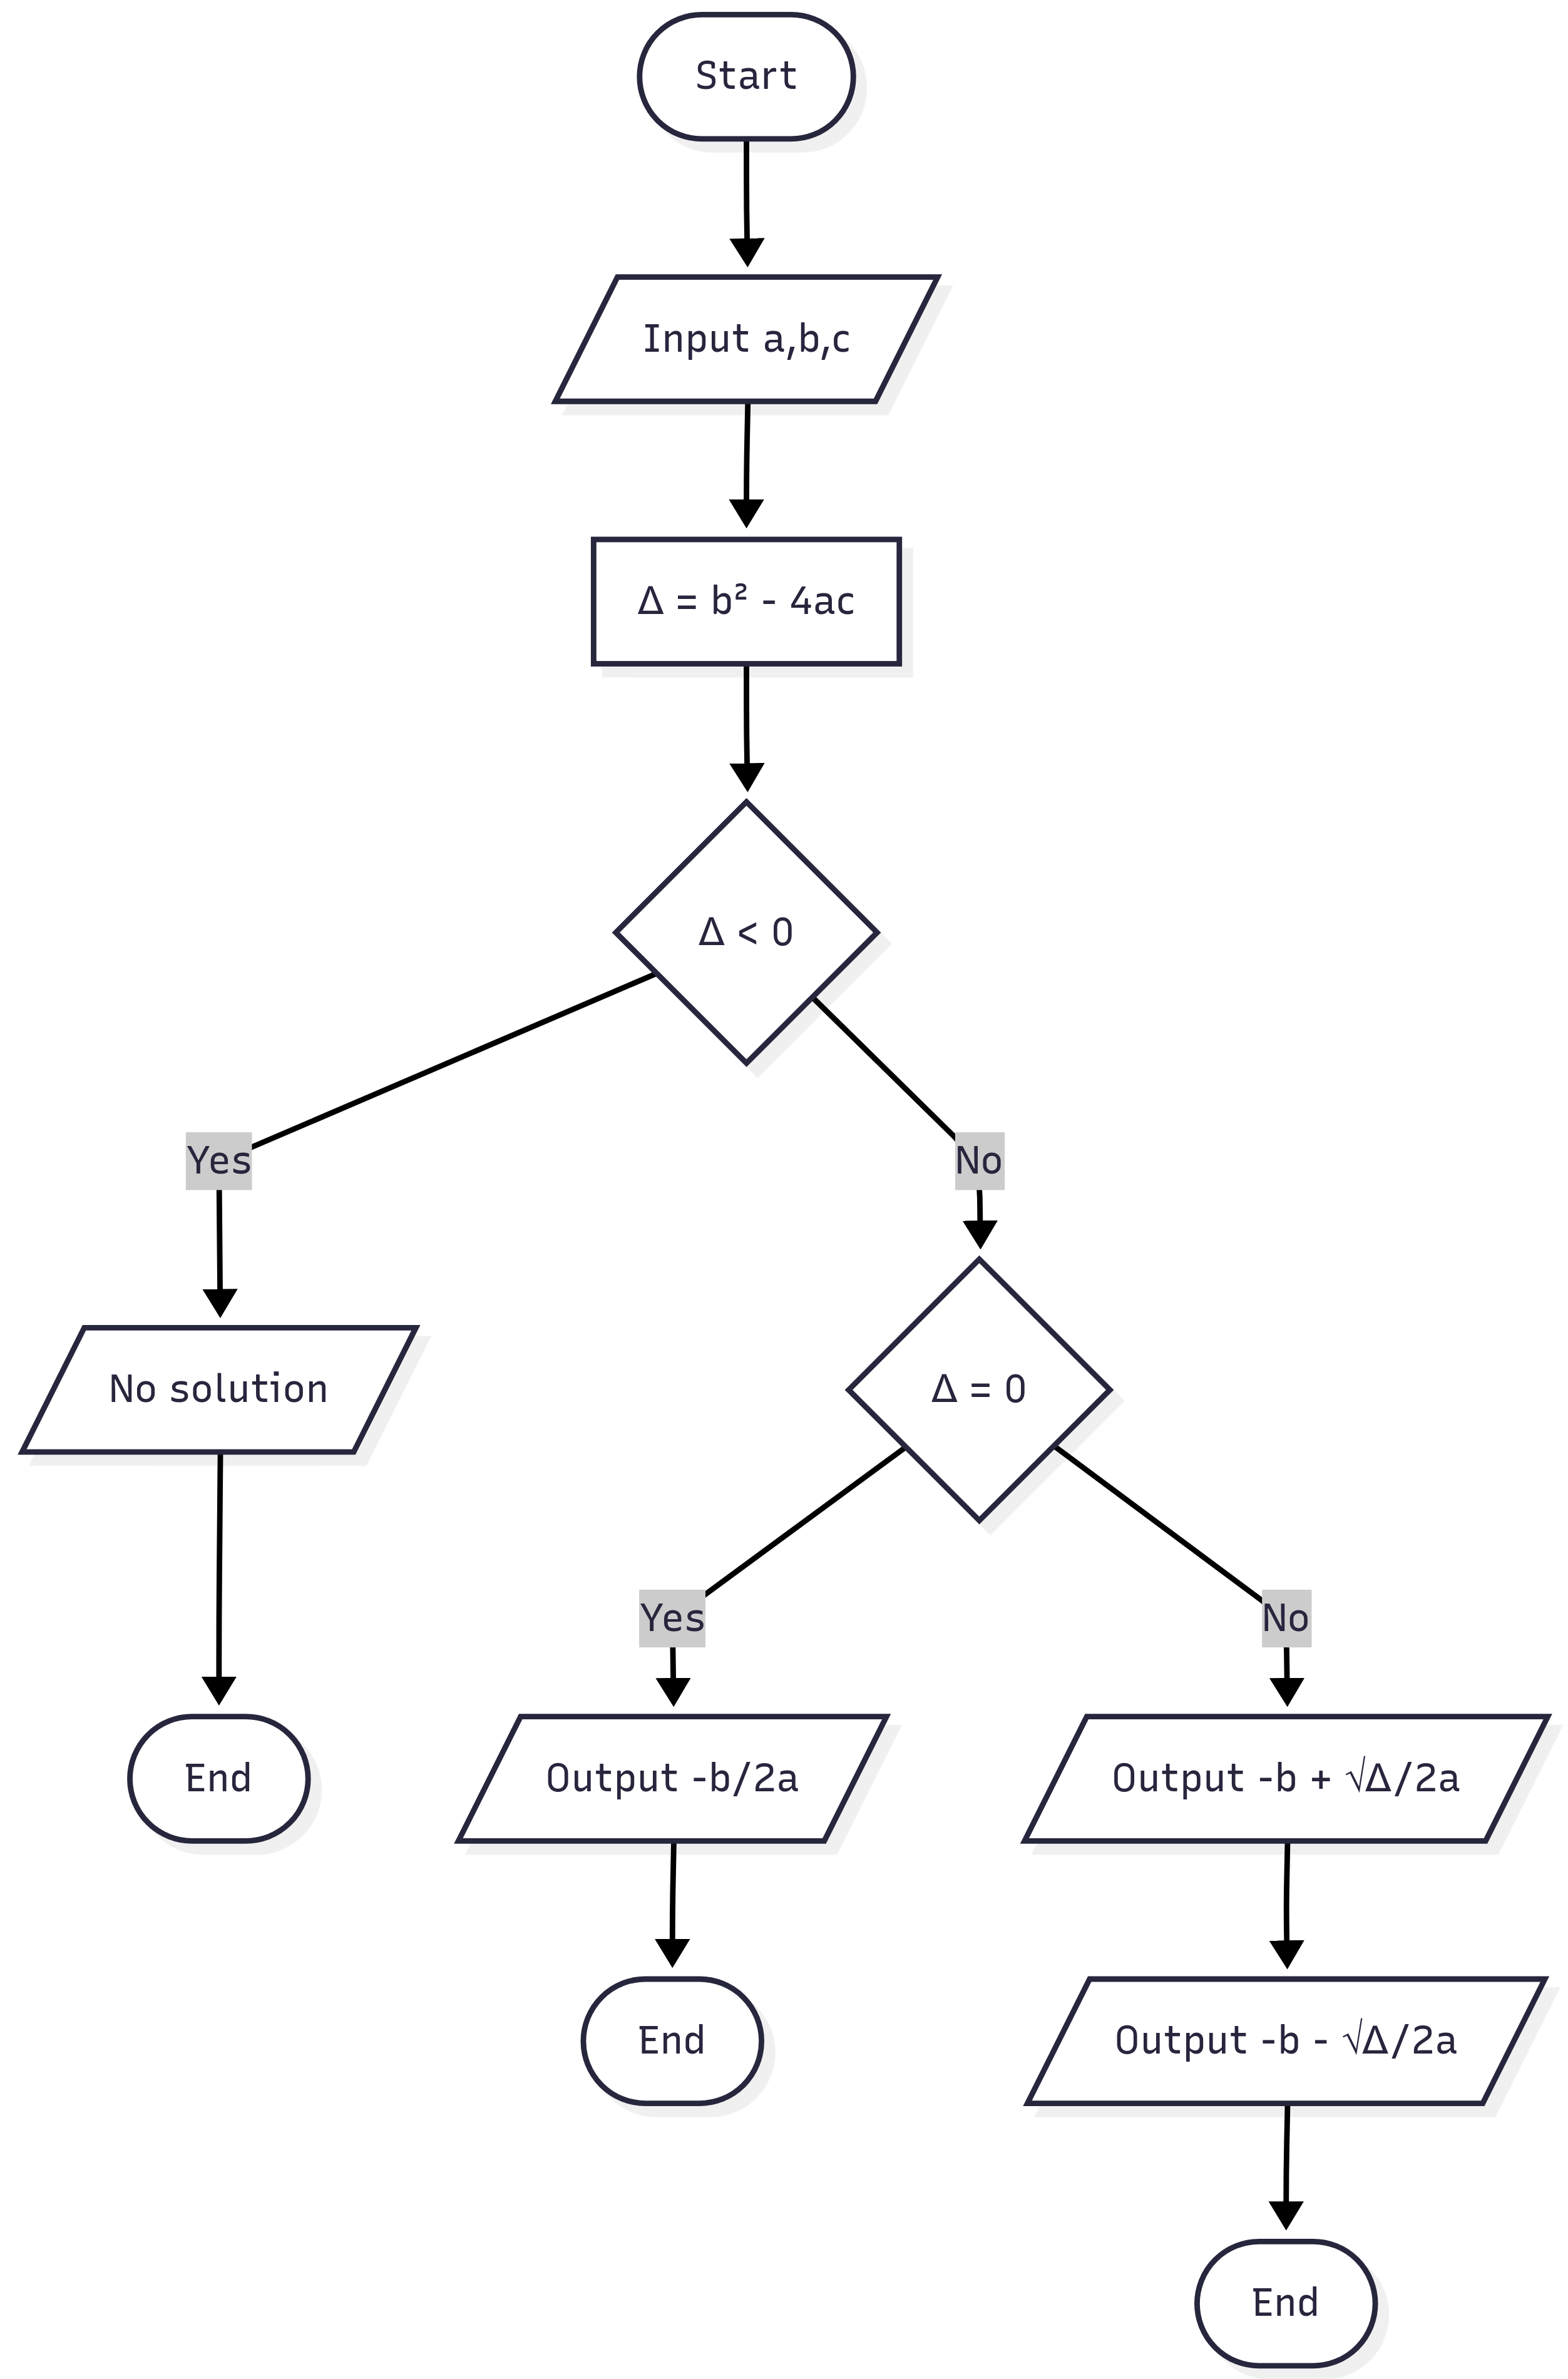
\includegraphics[height=4.35cm]{chat2.png} \\
		% Optional captions under each image
		(a) Our result & (b) GPT Mermaid & (c) GPT D2 \\
	\end{tabular}
	
	\vspace{1em}
	
	% Second row
	\begin{tabular}{ccc}
		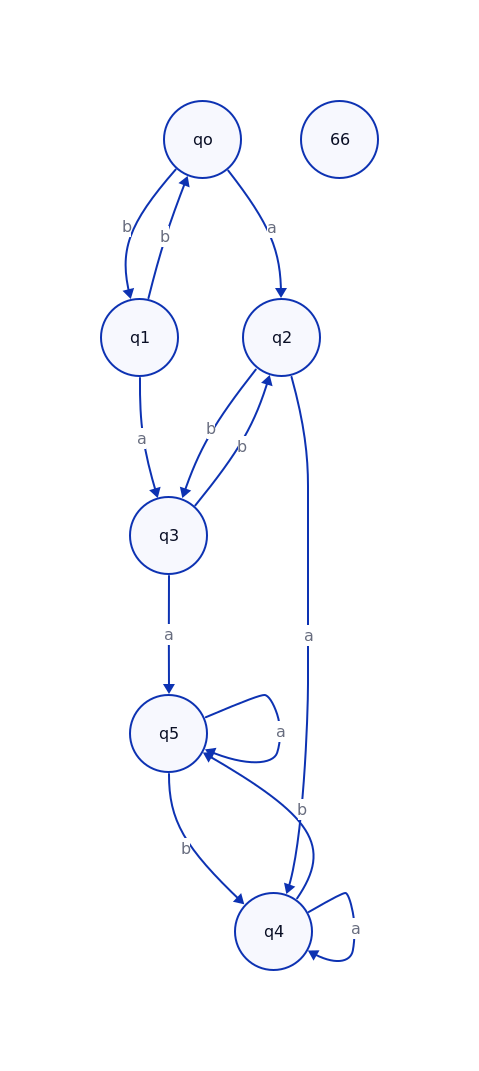
\includegraphics[height=5cm]{ex4.png} &
		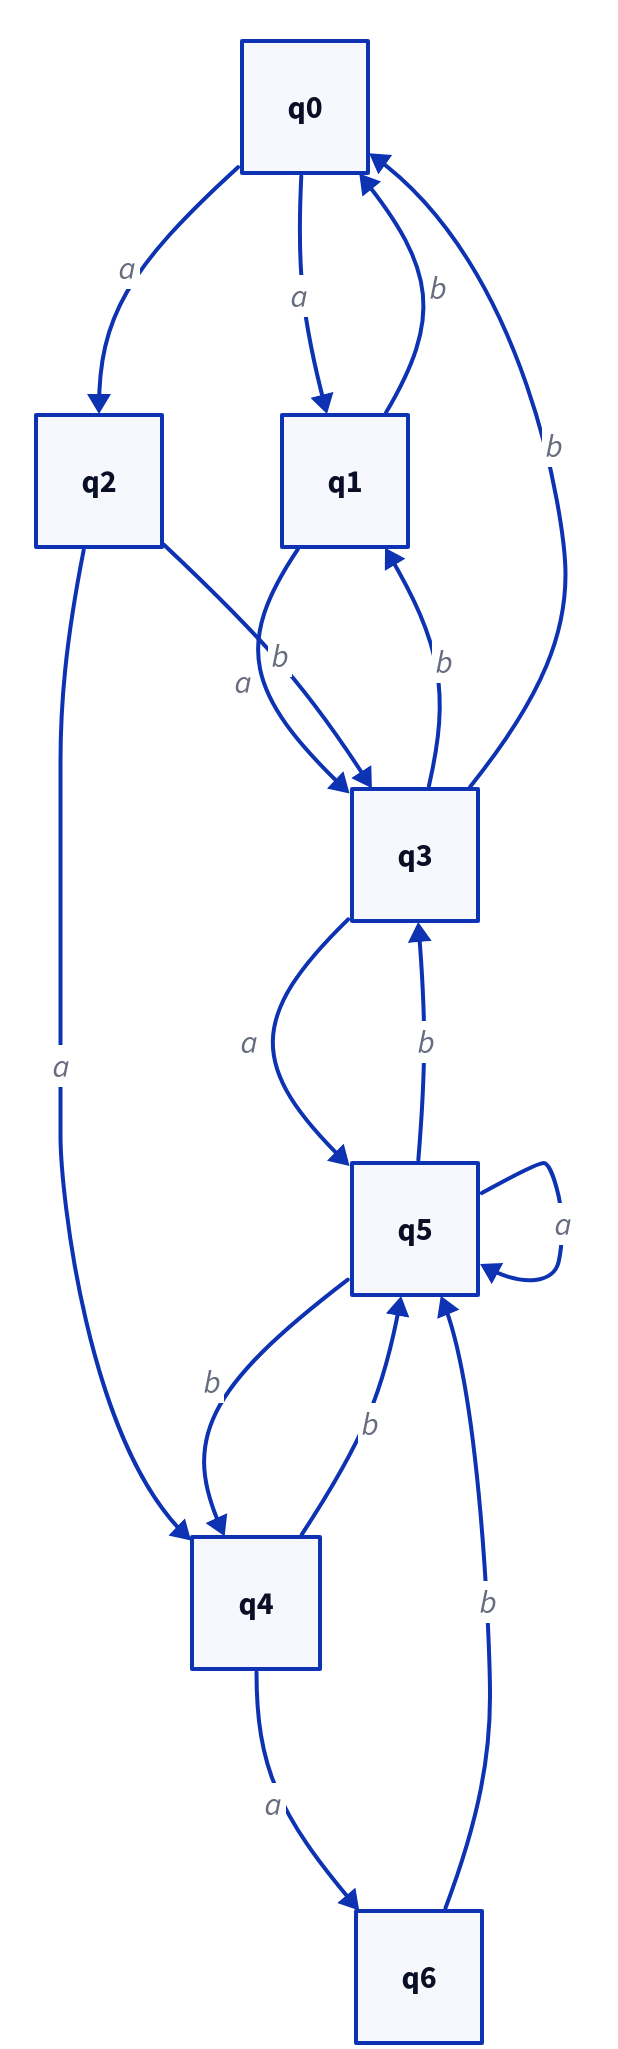
\includegraphics[height=5cm]{chat3.png} &
		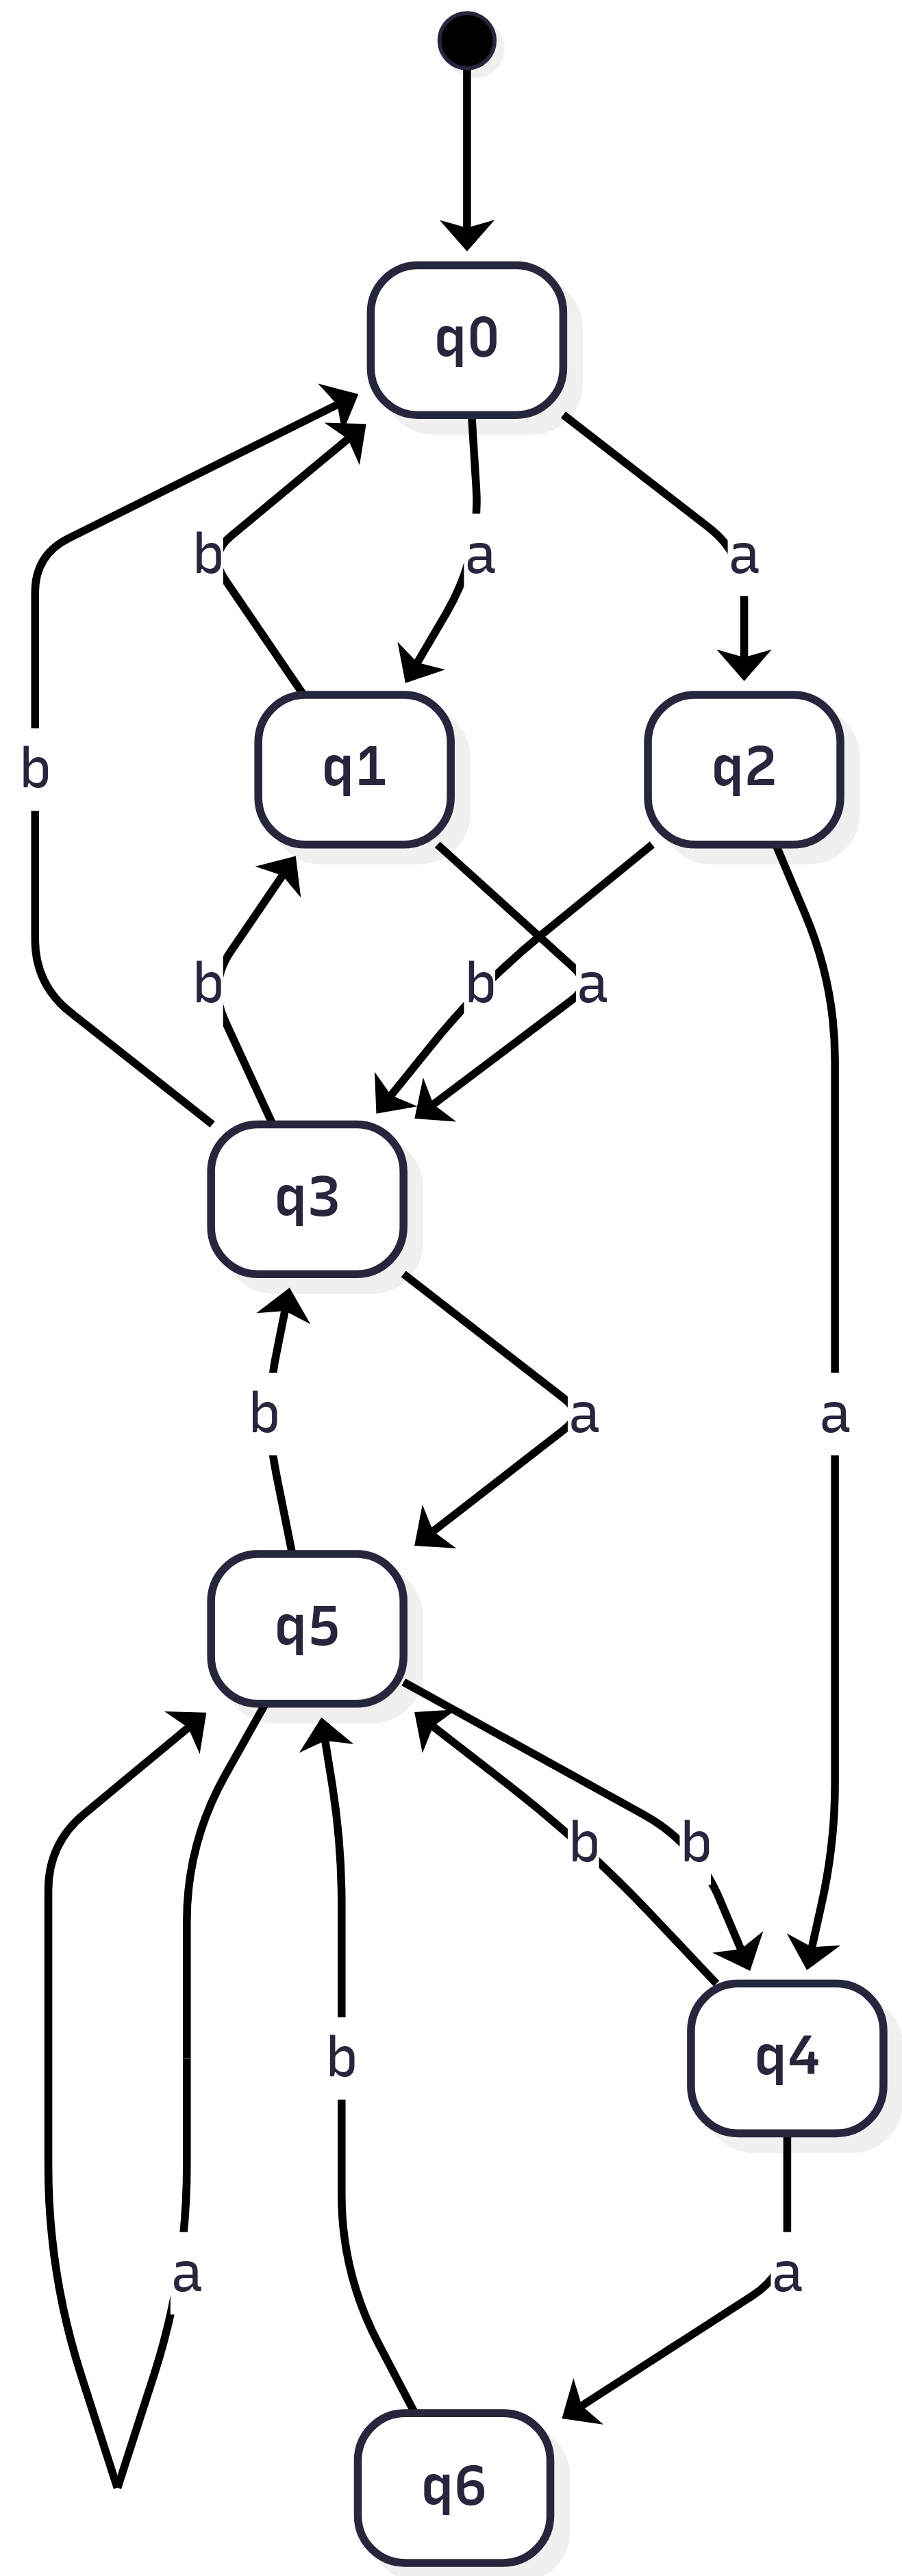
\includegraphics[height=5cm]{chat4.png} \\
		(d) Our result & (e) GPT Mermaid & (f) GPT D2 \\
	\end{tabular}
	
	\caption{Six vertically-oriented images arranged in two rows}
	\label{fig:chat}
	
\end{figure}

Another result we'd like to present is a comparison between D.I.A.G.R.A.M.'s results and what GPT-4o could give in zero-shot. The prompt given was the following: "The current image features a diagram. Analyze it and output the respective D2 and Mermaid script.". The results given (see Figure~\ref{fig:chat}) may be - at first glance - quite similar. However, some key differences arise. For instance, in diagrams (b), (e), (f), GPT isn't able to correctly output the shape of the nodes - whereas our net is capable of doing. Just like our net added a node instead of the self-arrow (see preceding paragraph), GPT isn't able to correctly recognize that portion of ink as a self-arrow (images (e), (f)). Another subtle difference - this time, not logical - can be seen in image (c): GPT created three different nodes, while the original image had only one.

\section{Conclusion and Future Work}
In this work, we introduced D.I.A.G.R.A.M., a system designed for the recognition and digitalization of visual diagrams. By combining deterministic algorithms with deep learning models, the system is capable of interpreting graphical input and converting it into structured, machine-readable formats. Our architecture demonstrates the feasibility of diagram understanding as a hybrid problem, leveraging both rule-based and learned components to achieve robustness and flexibility.

Despite the promising results, several opportunities remain for improvement. A key direction for future work is the parallelization of the extractor module, which currently represents a bottleneck in the processing pipeline. Efficient multi-threaded implementations could significantly speed up large-scale or real-time diagram analysis.

Additionally, to enhance portability and reproducibility, the system could benefit from containerization using Docker, particularly for managing CLI tools and Python dependencies. This would allow for more consistent deployment across diverse environments and simplify collaboration and maintenance.

Continued refinements in both the recognition pipeline and the system's usability will move us closer to a practical tool for academic, industrial, and educational use cases where diagram understanding and easy modeling is essential.

\newpage
\bibliographystyle{IEEEtran}
\bibliography{article}
\newpage

\begin{appendices}

\section{Double Clustering}
\label{double_clustering}
The first algorithmic approach proposed to solve this task - called \textit{Double Clustering} - was as follows: 
\begin{enumerate}
	\item Find the keypoints of the arrow using SIFT \cite{SIFT}.
	\item Apply a clustering algorithm to the image inside the bounding box, leveraging only the keypoints.
	\item Suppose that the biggest cluster belongs to the arrow; the other clusters are thought to contain useless elements for this task, and can be discarded.
	\item Find the two keypoints inside the arrow with maximum distance. Assume that these two points are closely related to the two ends of the arrow.
	\item Run a template matching procedure inside the two clusters to find the head of the arrow.
\end{enumerate}

For Step (1), we tried to employ both Spectral Clustering \cite{spectralclustering} (see Figure~\ref{fig:spectral_clustering}) and DBScan \cite{dbscan} (see Figure~\ref{fig:arrow_double_clustering_clusters}).

\begin{figure}[H]
	\centering
	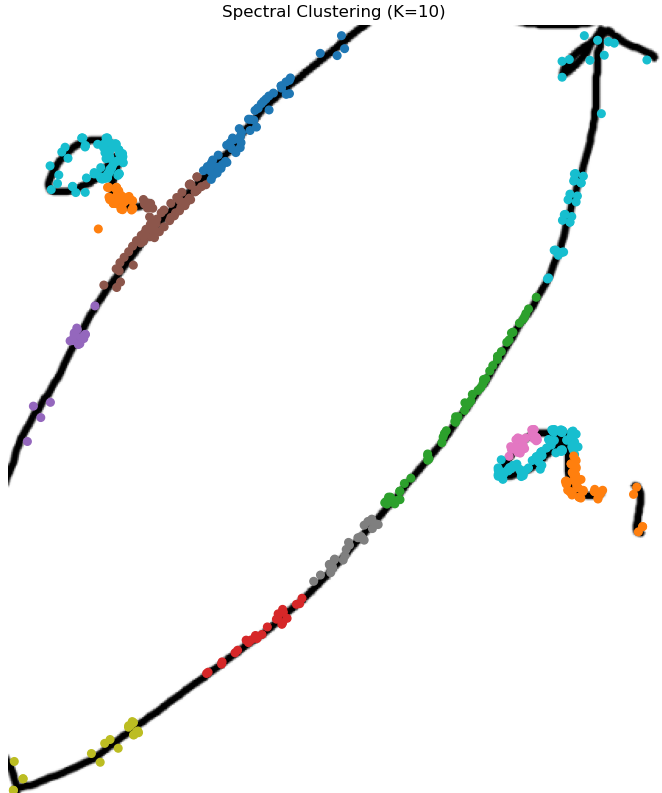
\includegraphics[width=150pt]{spectral_clustering.png}
	\caption{The result of Spectral Clustering to one instance of an arrow bounding box in our dataset.}
	\label{fig:spectral_clustering}
\end{figure}

\begin{figure}[H]
	\centering
	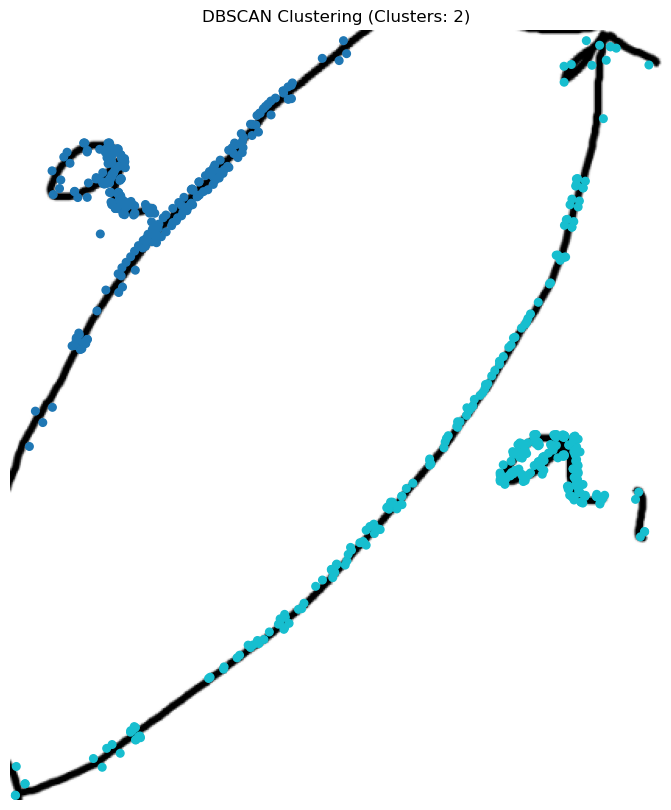
\includegraphics[width=150pt]{arrow_double_clustering_clusters.png}
	\caption{The result of DBScan to one instance of an arrow bounding box in our dataset.}
	\label{fig:arrow_double_clustering_clusters}
\end{figure}

For Step (3), we used SIFT \cite{SIFT} in order to find keypoints and some descriptors for them - necessary for the later template matching.
During Step (4), we were able to correctly deduce the overall direction of the arrow (see Figure~\ref{fig:arrow_double_clustering_direction}).

\begin{figure}[H]
	\centering
	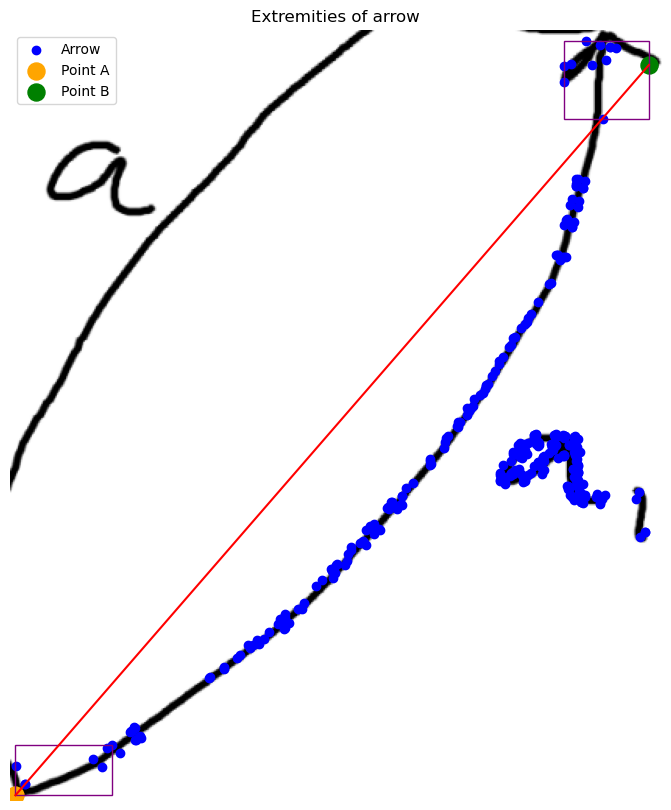
\includegraphics[width=150pt]{arrow_double_clustering_direction.png}
	\caption{The estimated direction of the arrow, finding the points that maximize the distance inside the cluster.}
	\label{fig:arrow_double_clustering_direction}
\end{figure}

For Step (5), we had previously hand-picked some templates (see Figure~\ref{fig:templates}).

\begin{figure}[H]
	\centering
	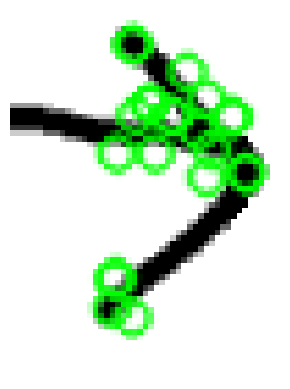
\includegraphics[width=50pt, height=60pt]{templates.png}
	\caption{An example of hand-picked template with SIFT descriptors.}
	\label{fig:templates}
\end{figure}

However, this approach didn't work as expected (see Figure~\ref{fig:template_matching_fail}). In particular, it never worked around self arrows: the maximized distance inside one of the two clusters is never between the tail and the head of the arrow (see Figure~\ref{fig:selfarrowdc}).

\begin{figure}[H]
	\centering
	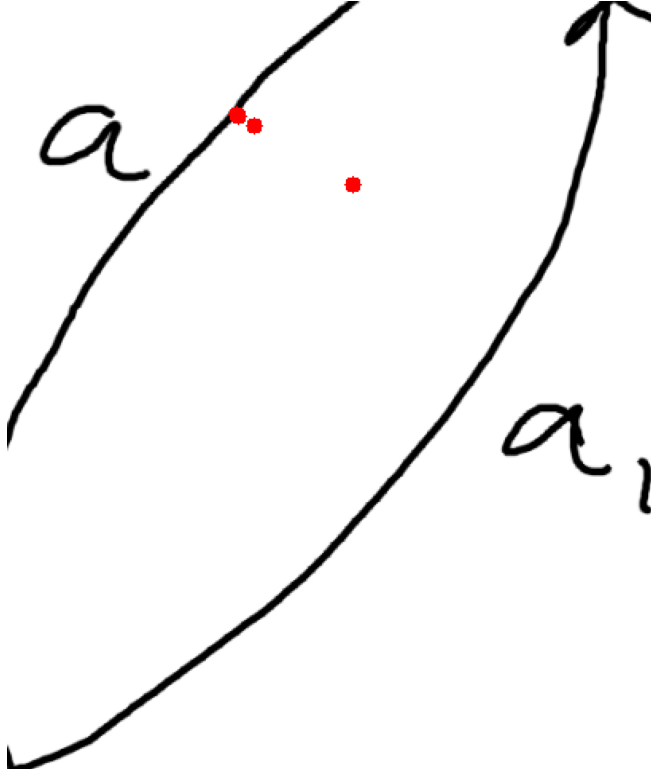
\includegraphics[width=150pt]{template_matching_fail.png}
	\caption{The overall result of the algorithm.}
	\label{fig:template_matching_fail}
\end{figure}

\begin{figure}[H]
	\centering
	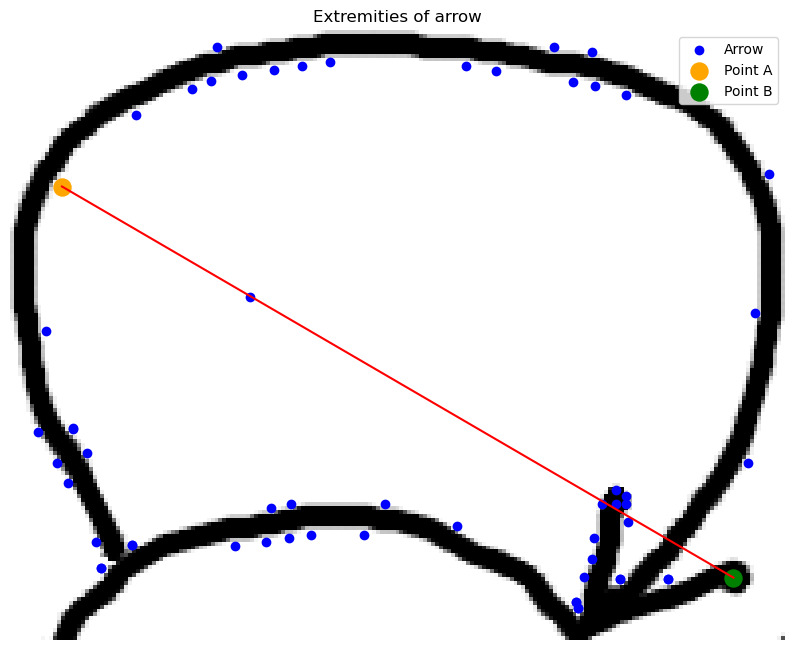
\includegraphics[width=150pt]{selfarrowdc.jpg}
	\caption{An instance which explains why the self-arrow's tail and head are not correctly recognized.}
	\label{fig:selfarrowdc}
\end{figure}

\section{ArrowNet}
\label{arrow-net}
This second approach for determining an arrow's orientation was inspired by UNet \cite{unet}. The core idea was to segment an arrow's bounding box, and to use a specific CNN to try and determine the arrow's head point and the arrow's tail point. This downsampling-upsampling network is called \textbf{ArrowNet} and its specifics can be found in Table~\ref{table:arrownet}.

\begin{table}[htbp]
	\centering
	\caption{ArrowNet Architecture Details}
	\label{tab:arrownet}
	\begin{tabular}{|l|l|l|l|l|}
		\hline
		\textbf{Stage} & \textbf{Layer} & \textbf{Out Ch} & \textbf{Operations} \\
		\hline
		\multirow{3}{*}{Encoder} 
		& Encoder1 & $32$ & Double Conv Block \\
		& MaxPool & $32$ & $2 \times 2$ MaxPooling \\
		& Encoder2 & $64$ & Double Conv Block \\
		\hline
		Bottleneck 
		& MaxPool+Bottleneck & $128$ & MaxPool+Double Conv \\
		\hline
		\multirow{4}{*}{Decoder}
		& Upsampling2 & $64$ & Transpose Conv Block \\
		& Skip + Decoder2 & $64$ & Concat + Double Conv \\
		& Upsampling1 & $32$ & Transpose Conv Block \\
		& Skip + Decoder1 & $32$ & Concat + Double Conv \\
		\hline
		Output & Output Conv & $2$ & $1 \times 1$ Convolution \\
		\hline
	\end{tabular}
	\label{table:arrownet}
\end{table}

The entire architecture is composed of three main building blocks:

\begin{enumerate}
\item \textbf{Double Convolution Block:} Each double convolution block applies two consecutive $3 \times 3$ convolutions with padding 1, followed by batch normalization, and a ReLU activation after each convolution. This should preserve spatial dimensions while increasing feature depth.

\item \textbf{Upsampling Block:} The upsampling blocks use $2 \times 2$ transposed convolutions with stride 2, followed by batch normalization and ReLU activation.

\item \textbf{Skip Connections:} The architecture employs skip connections that concatenate feature maps from the encoder path with corresponding decoder features.

\end{enumerate}

The two output float channels of ArrowNet should have been used to predict, in a given position: $1$ if the head's point is in a certain position, $0$ else; $1$ if the tail's point is in a certain position, $0$ else - for the first and second channel respectively.

\begin{figure}[H]
	\centering
	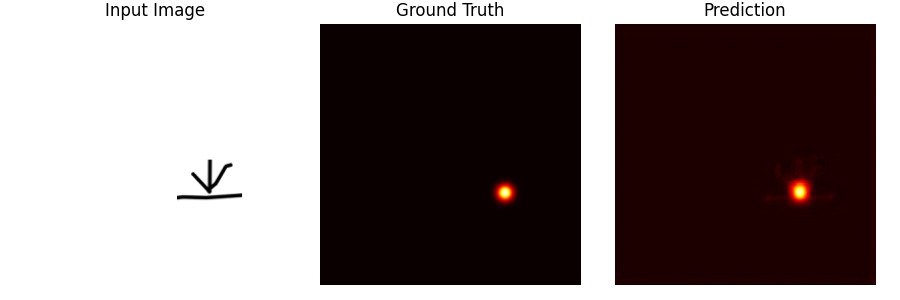
\includegraphics[width=225pt, height=75pt]{arrownet1.jpg}
	\caption{Some results for arrow's head reconstruction.}
	\label{fig:arrownet1}
\end{figure}

Due to the low quality of synthetic samples provided, the network is unable to correctly distinguish between an arrow's head and tail. In particular, the network overfitted and simply detected as correct the presence of black ink.

\section{The Classification Network}
\label{classification_net}

The \textbf{Classification Network} is a lightweight convolutional neural network, suited for processing grayscale images. The architecture is composed of convolutional feature extraction layers followed by fully connected classification layers. Some specifics about it can be found in Table~\ref{tab:classification-architecture}.

\begin{table}[h]
	\centering
	\caption{Classification Network Details}
	\label{tab:classification-architecture}
	\begin{tabular}{|c|c|c|c|}
		\hline
		\textbf{Layer Type} & \textbf{Out Channels} & \textbf{Kernel Size} & \textbf{Pool Kernel Size} \\
		\hline 
		Conv & 8 & 2 & 3 \\
		Conv & 16 & 2  & 3 \\
		Conv & 24 & 3  & 2 \\
		\hline
		\textbf{Layer Type} & \textbf{Out Features} & \textbf{Droput Rate} & \textbf{Activation Function} \\
		\hline 
		Linear & 2048 & 0.2 & ReLU \\
		Linear & 128 & 0.2 & ReLU \\
		Linear & 3 & 0.2 & ReLU \\
		\hline
	\end{tabular}
\end{table}

Each convolutional layer, is followed by a ReLU activation function, a layer which applies batch normalization and by a MaxPooling layer.

\end{appendices}

\end{document}
